Software guards our secrets, our money, our intellectual property,
our reputation \cite{covern}.  We entrust personal and
corporate information to software which works in an \emph{open} world, 
where  it interacts with 
third party software of unknown provenance, possibly buggy and potentially malicious.

This means we need our software to be \emph{robust}.
We expect software to behave correctly even if  used 
by erroneous or malicious third parties.
 We expect that our bank will only make payments 
from our account if instructed by us, or by somebody we have authorised, 
that space on a web given to an advertiser will not be used
to obtain access to our bank details \cite{cwe}, or that an
airline will not sell more tickets than the number of seats.
The importance of robustness has led to the design of many programming
language mechanisms to help developers write robust programs:
constant fields, private methods, ownership \cite{ownalias}
as well as the object capability paradigm \cite{MillerPhD},
and its adoption in  web systems
\cite{CapJavaHayesAPLAS17,CapNetSocc17Eide,DOCaT14}, and programming languages such as Newspeak
\cite{newspeak17}, Dart \cite{dart15},
Grace \cite{grace,graceClasses}, and Wyvern \cite{wyverncapabilities}.

While such programming language mechanisms make it \textit{possible} to write robust
programs, they cannot \textit{ensure} that programs are robust.
Ensuring robustness is difficult because it means 
different things for different systems: perhaps
that critical operations should only be invoked with the requisite authority;
perhaps that sensitive personal information should not be leaked; 
or perhaps that resource belonging to one user should not be consumed by another.
%
To be able to ensure robustness, we need ways to specify what robustness means for a 
particular program, and ways to demonstrate that the particular program 
adheres to its specific robustness requirements.

There has been a plethora of work on the specification and verification of the
functional correctness of programs. Such specifications describe what are
essentially \emph{sufficient} conditions for some
effect to happen. For example, if you have enough funds and make a payment request to your bank, money will be transferred
and as a result your balance funds will be reduced: enough funds and the payment request is a sufficient condition for the
reduction of funds.
Often, however, we are also interested in \emph{necessary conditions}:
guarantees about things that will  \emph{not} happen.
%
For example, you  probably 
want to be assured that no reduction in your bank balance will take place unless you have
explicitly requested it. Similarly, medical patients want  to be assured  that   their health data will not be sent to  their employer  
unless they authorised the release:
the patient's explicit authorisation is the
necessary condition for the communication of health data --- under no
other circumstances should the data be communicated.

Fig. \ref{fig:NecessaryAndSuff} shows
the difference between sufficient and necessary conditions. 
We
represent  all possible states through black dots, and place all  initial states in the grey box.
Sufficient conditions are described on a per-function basis: 
a function call in a certain state leads to another state
-- in part (a) we indicate different functions through different shades of blue and green. 
Necessary conditions, on the other hand, are about the behaviour of a component
as a whole, 
and describe what is guaranteed not to happen;
in part (b) we place  states that are guaranteed not to be reached in yellow boxes
with dotted outlines,
and indicate transitions that are guaranteed not to happen through
yellow, dotted arrows.


%With the old diagrams
% \begin{tabular}{ccccc}
%\begin{minipage}{0.25\textwidth}
% 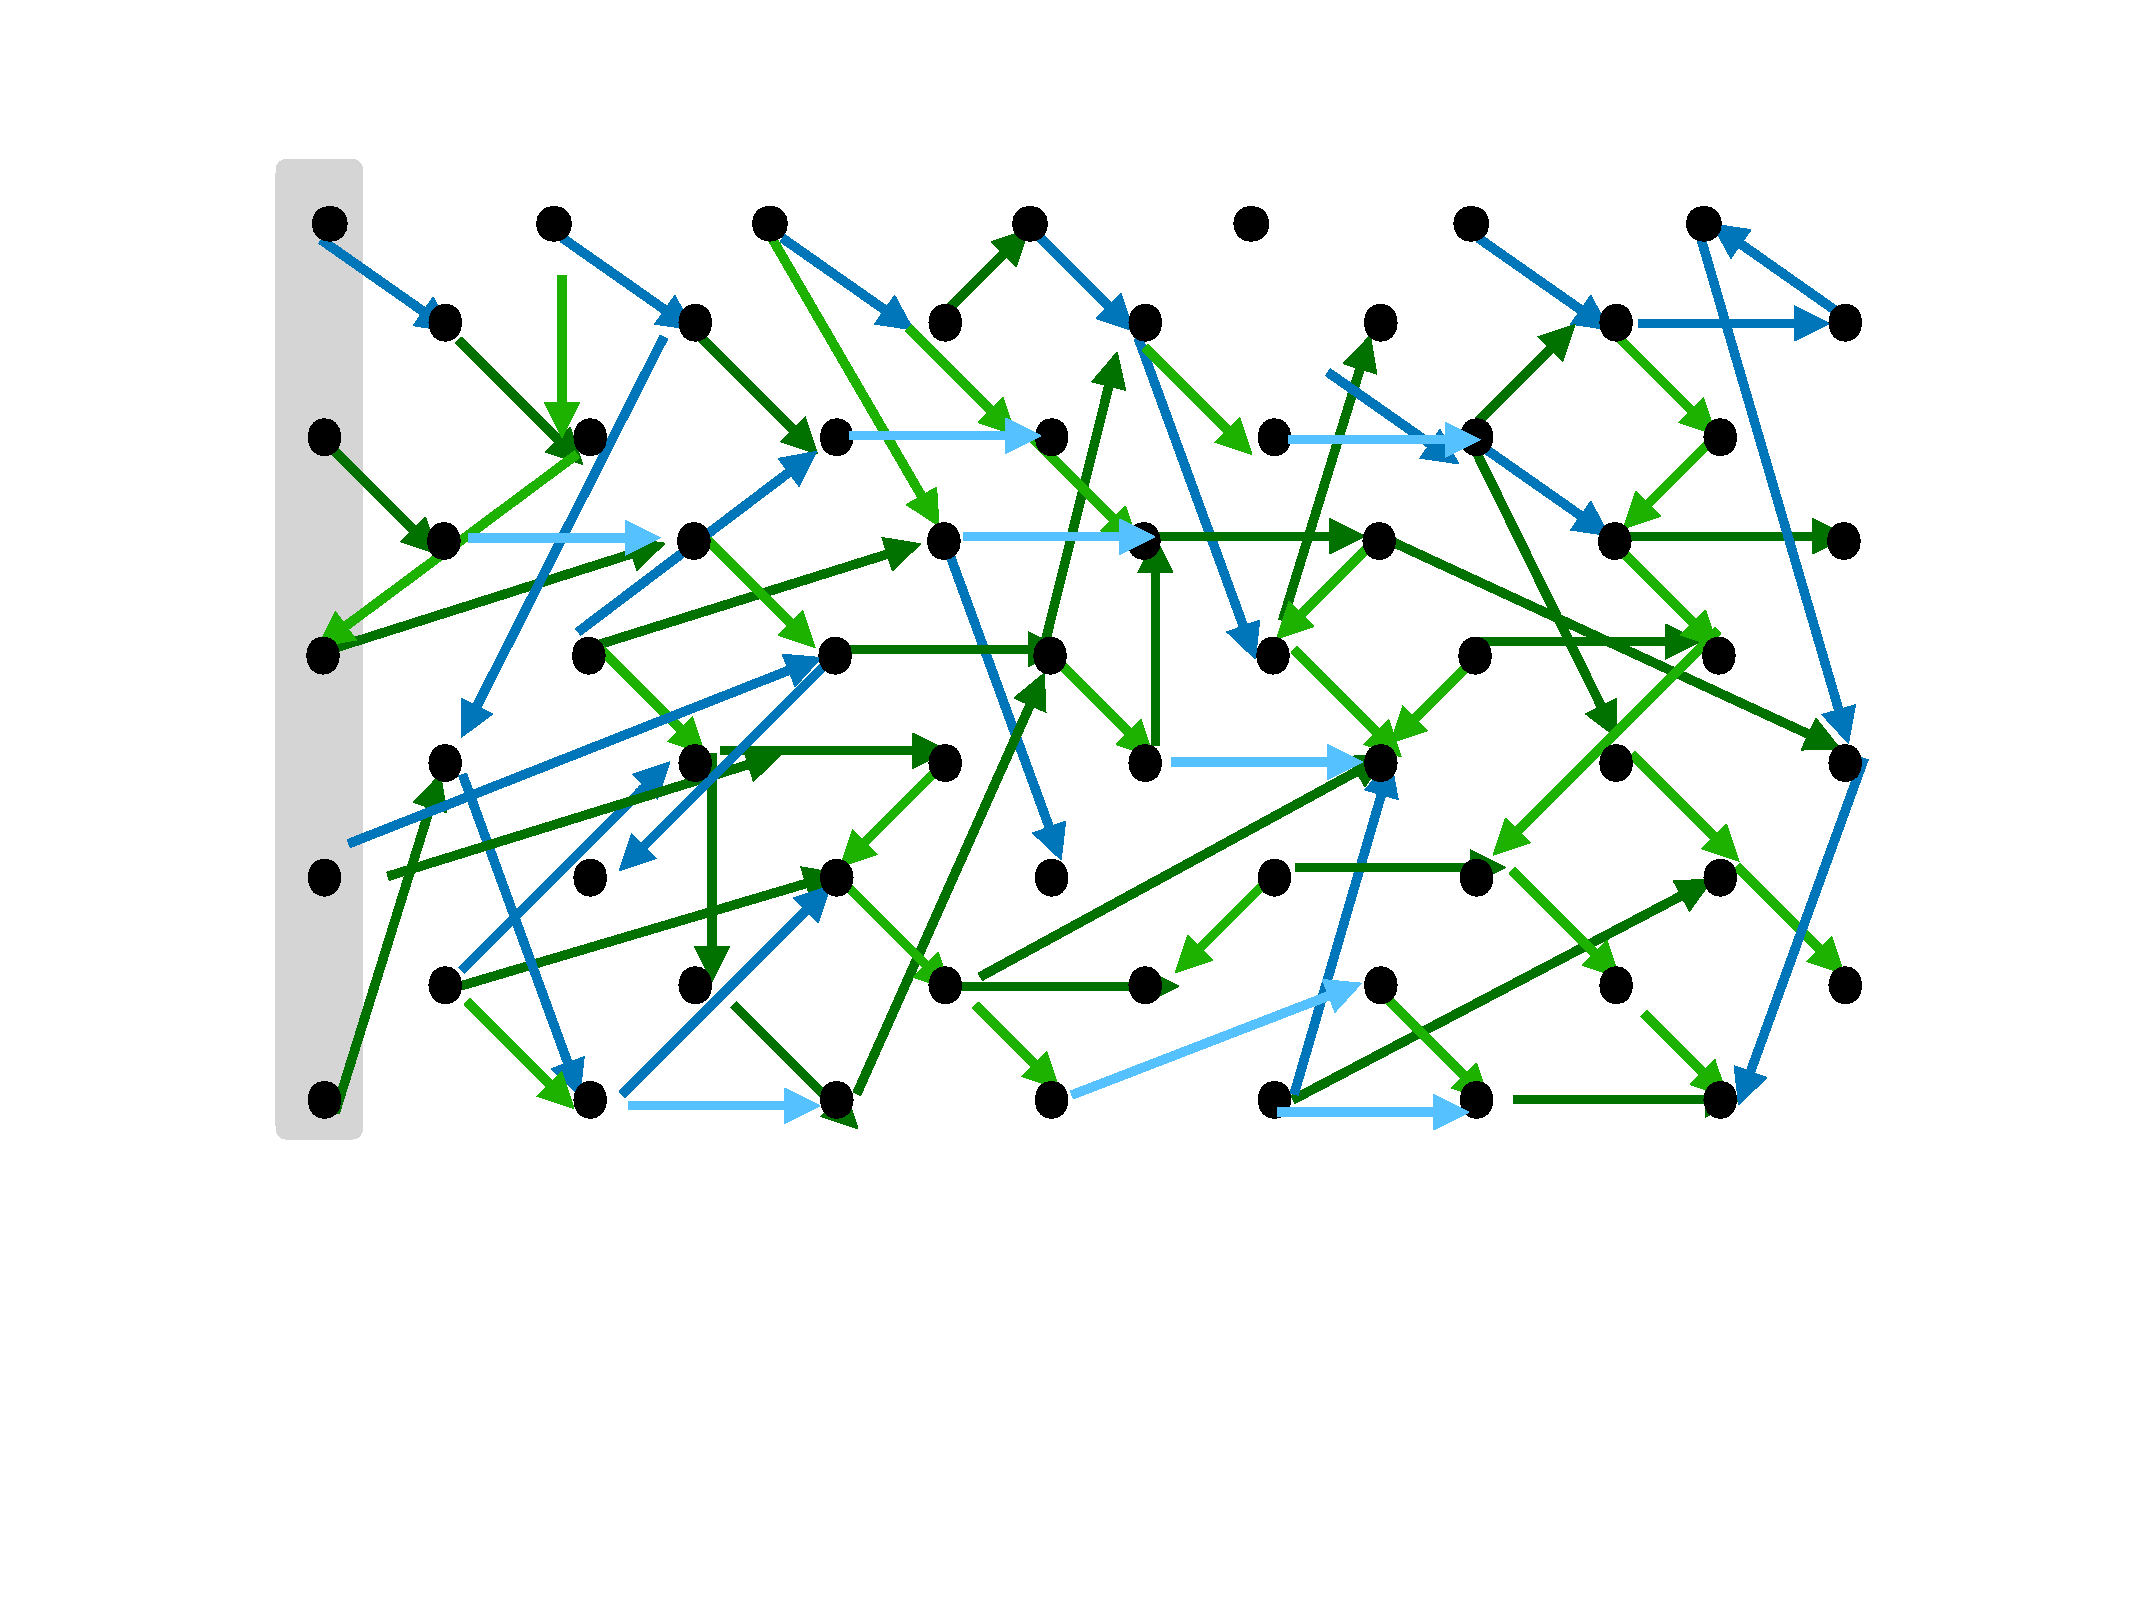
\includegraphics[width=\linewidth, trim=250  320 260 60,clip]{diagrams/neccSuff_yellow_A.pdf}
%\end{minipage}
% & \ \ \ & 
%\begin{minipage}{0.25\textwidth}
% 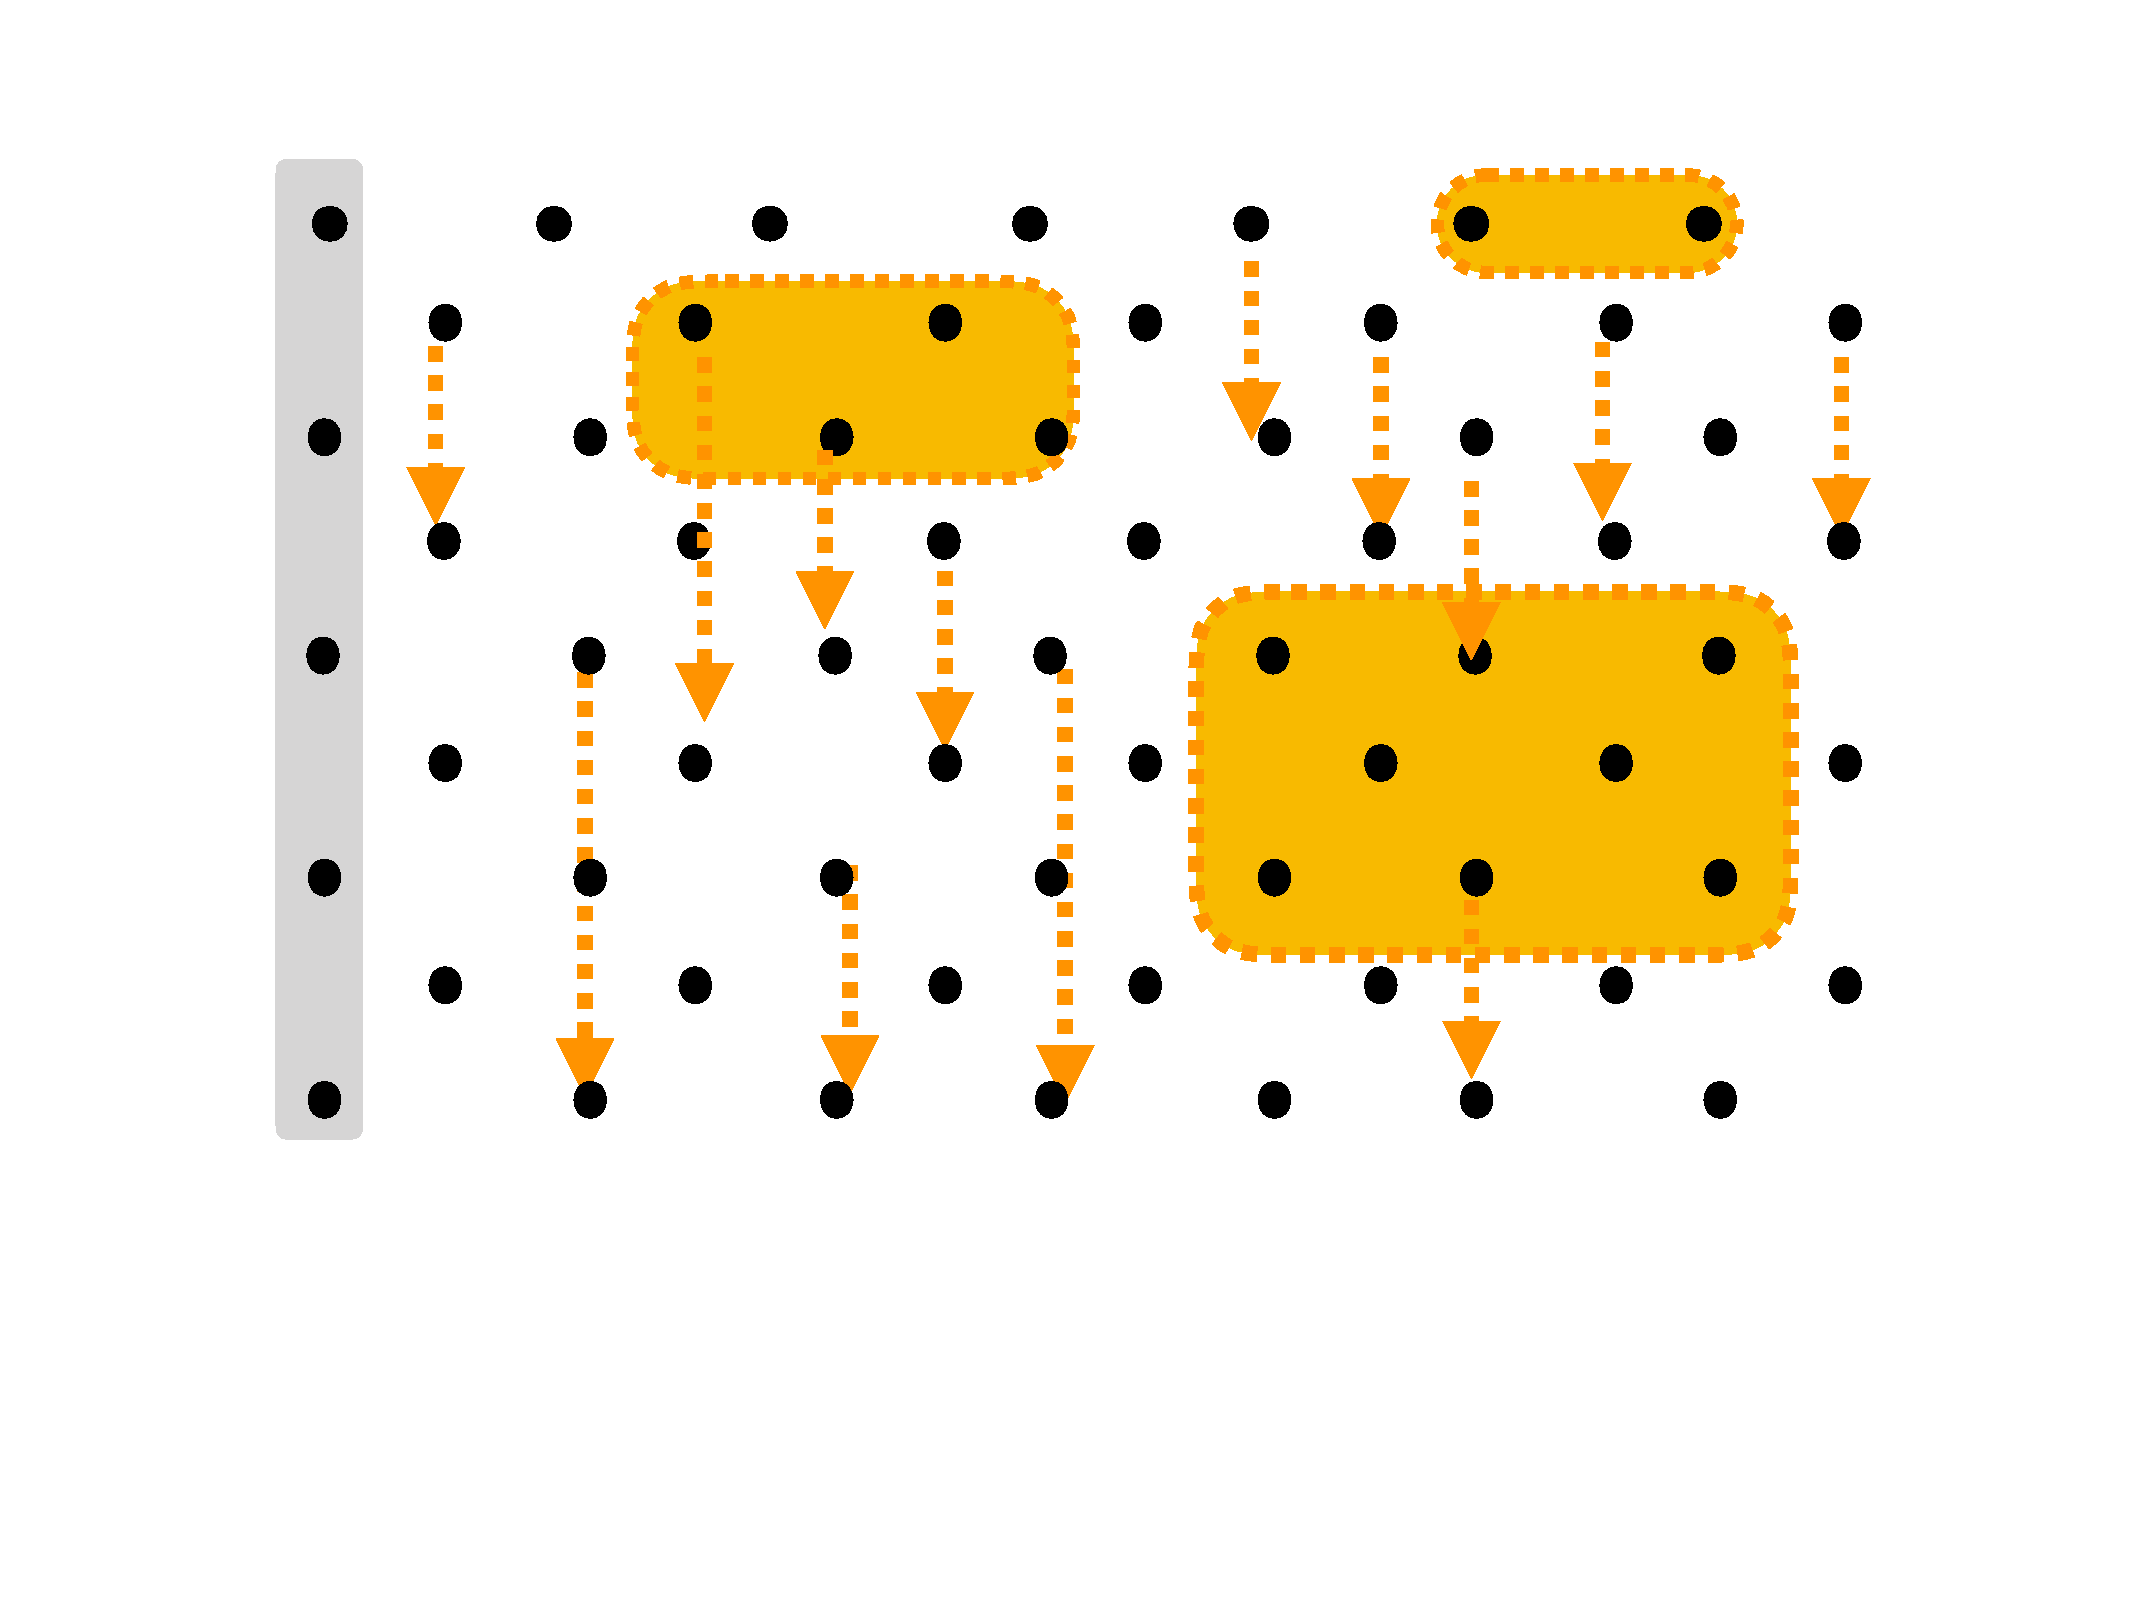
\includegraphics[width=\linewidth, trim=250  320 260 60,clip]{diagrams/neccSuff_yellow_B.pdf}
%\end{minipage}
% & \ \ \ &
%\begin{minipage}{0.25\textwidth}
% 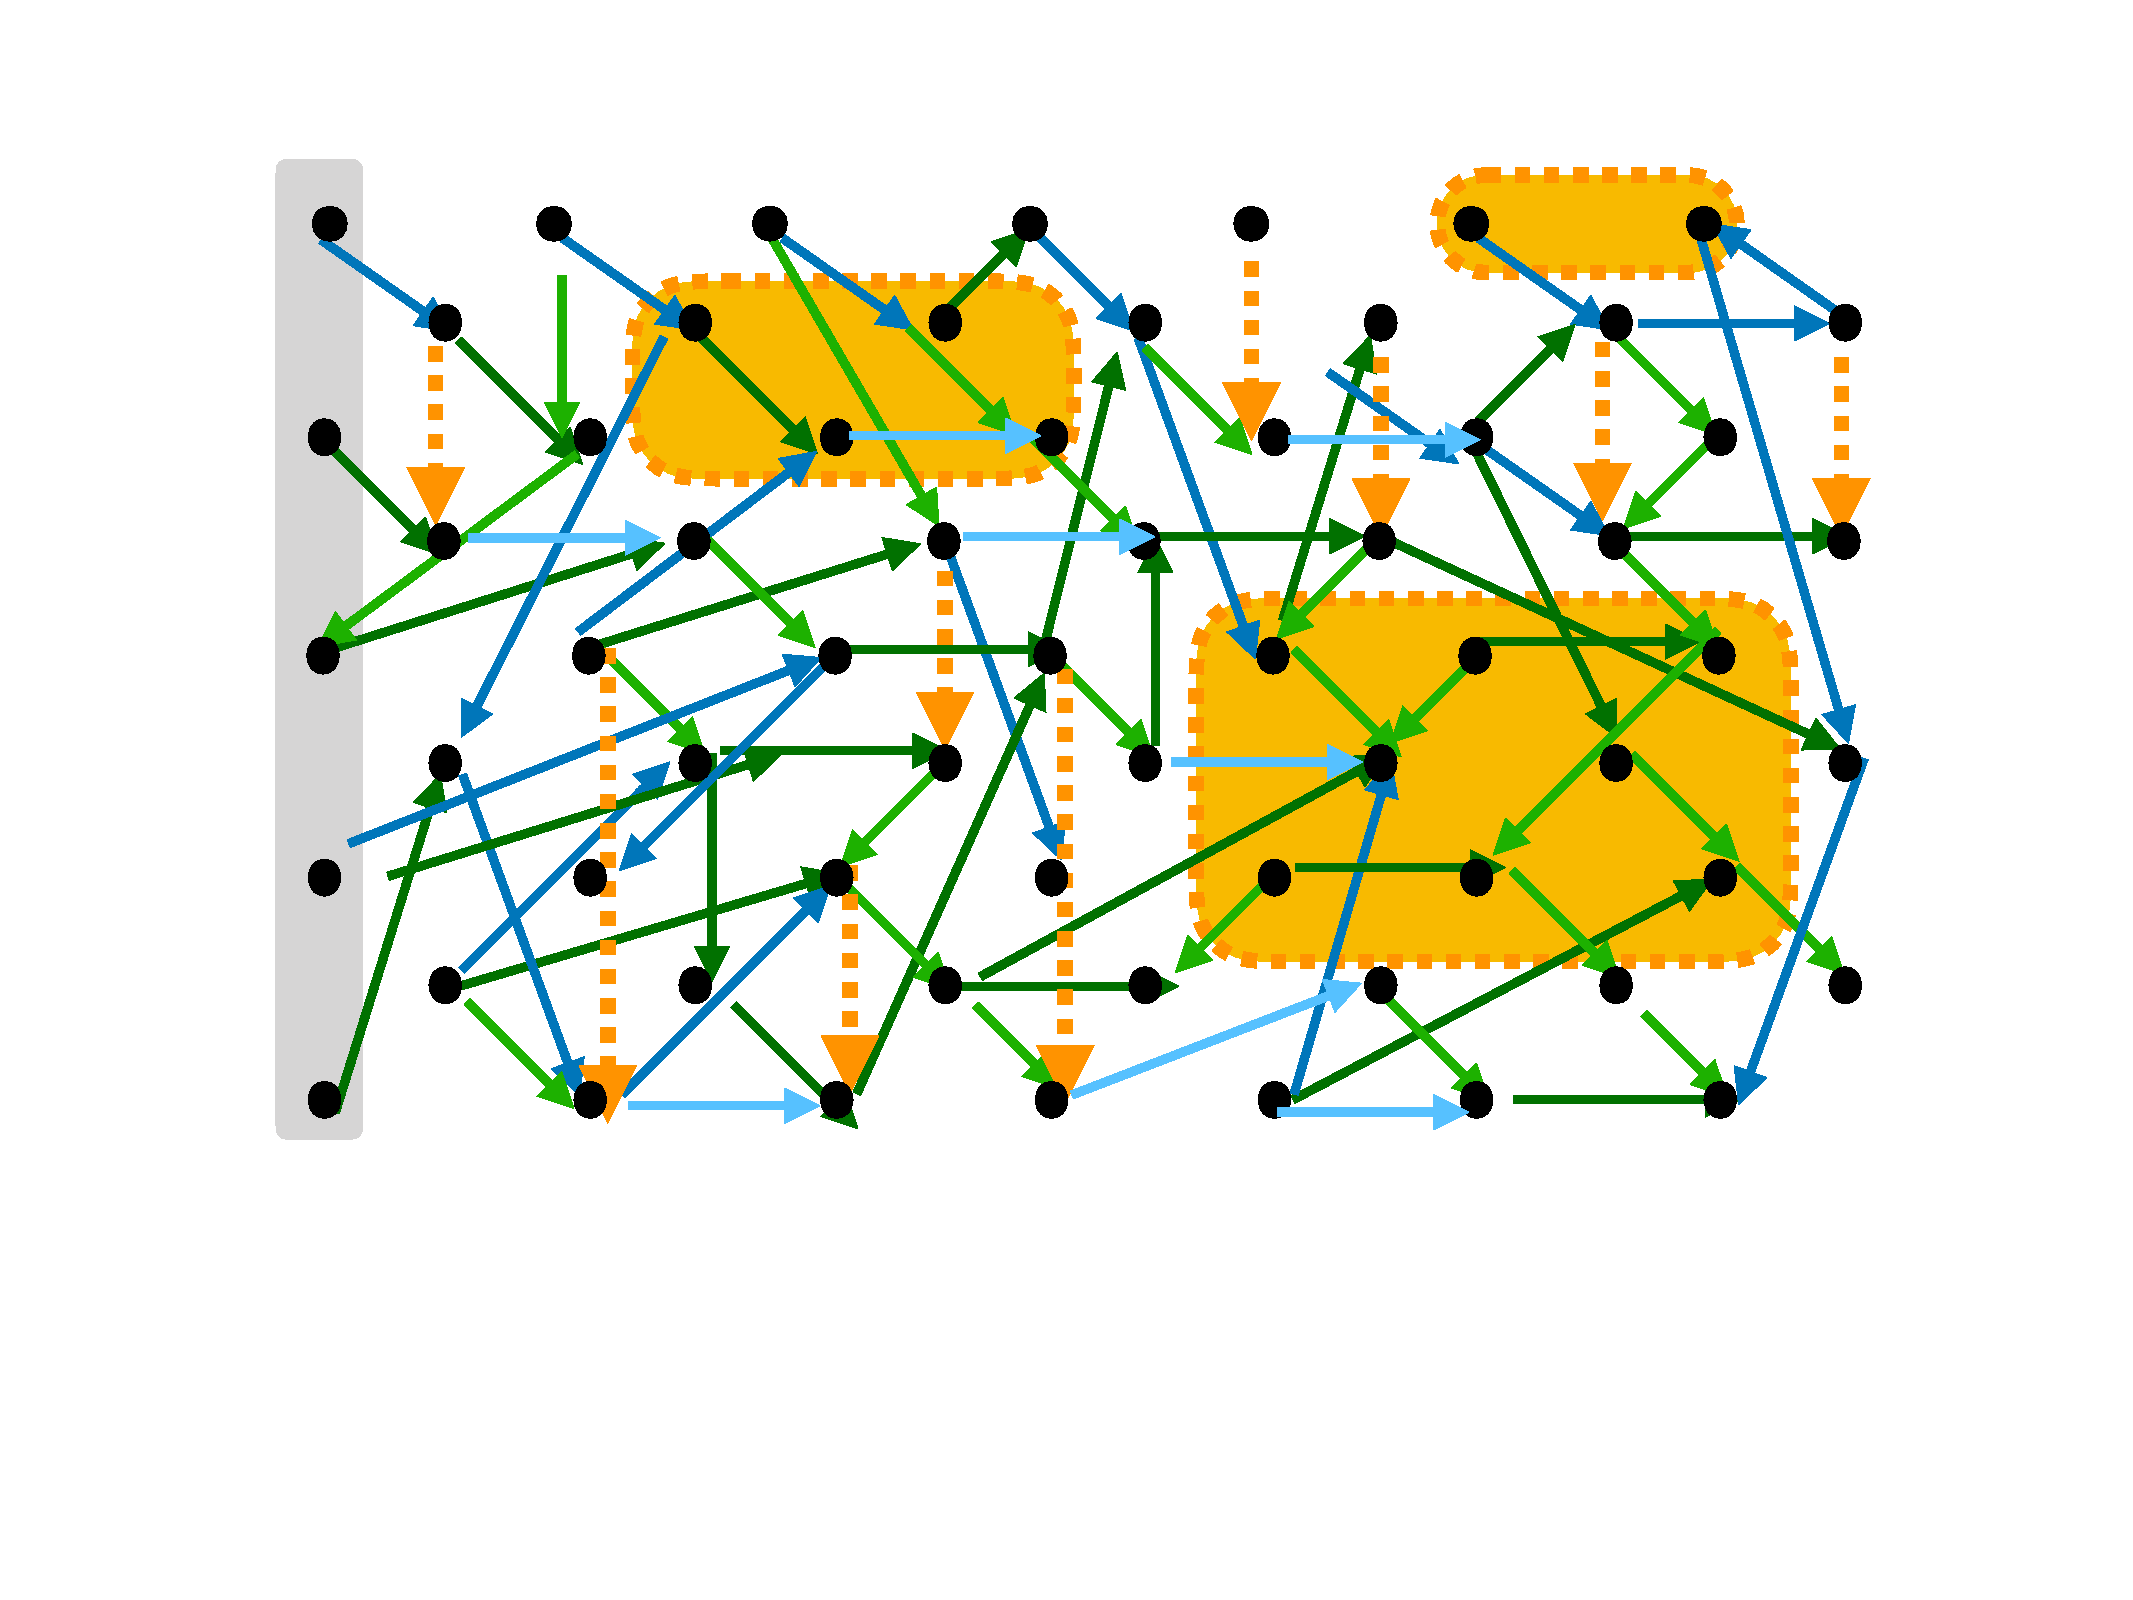
\includegraphics[width=\linewidth, trim=250  320 260 60,clip]{diagrams/neccSuffYellowAll.pdf}
% \end{minipage}
 


%  THE DIAGRAM WITH MIORE LINES IN C
%\begin{figure}[htb]
% \begin{tabular}{clclc}
%\begin{minipage}{0.29\textwidth}
% 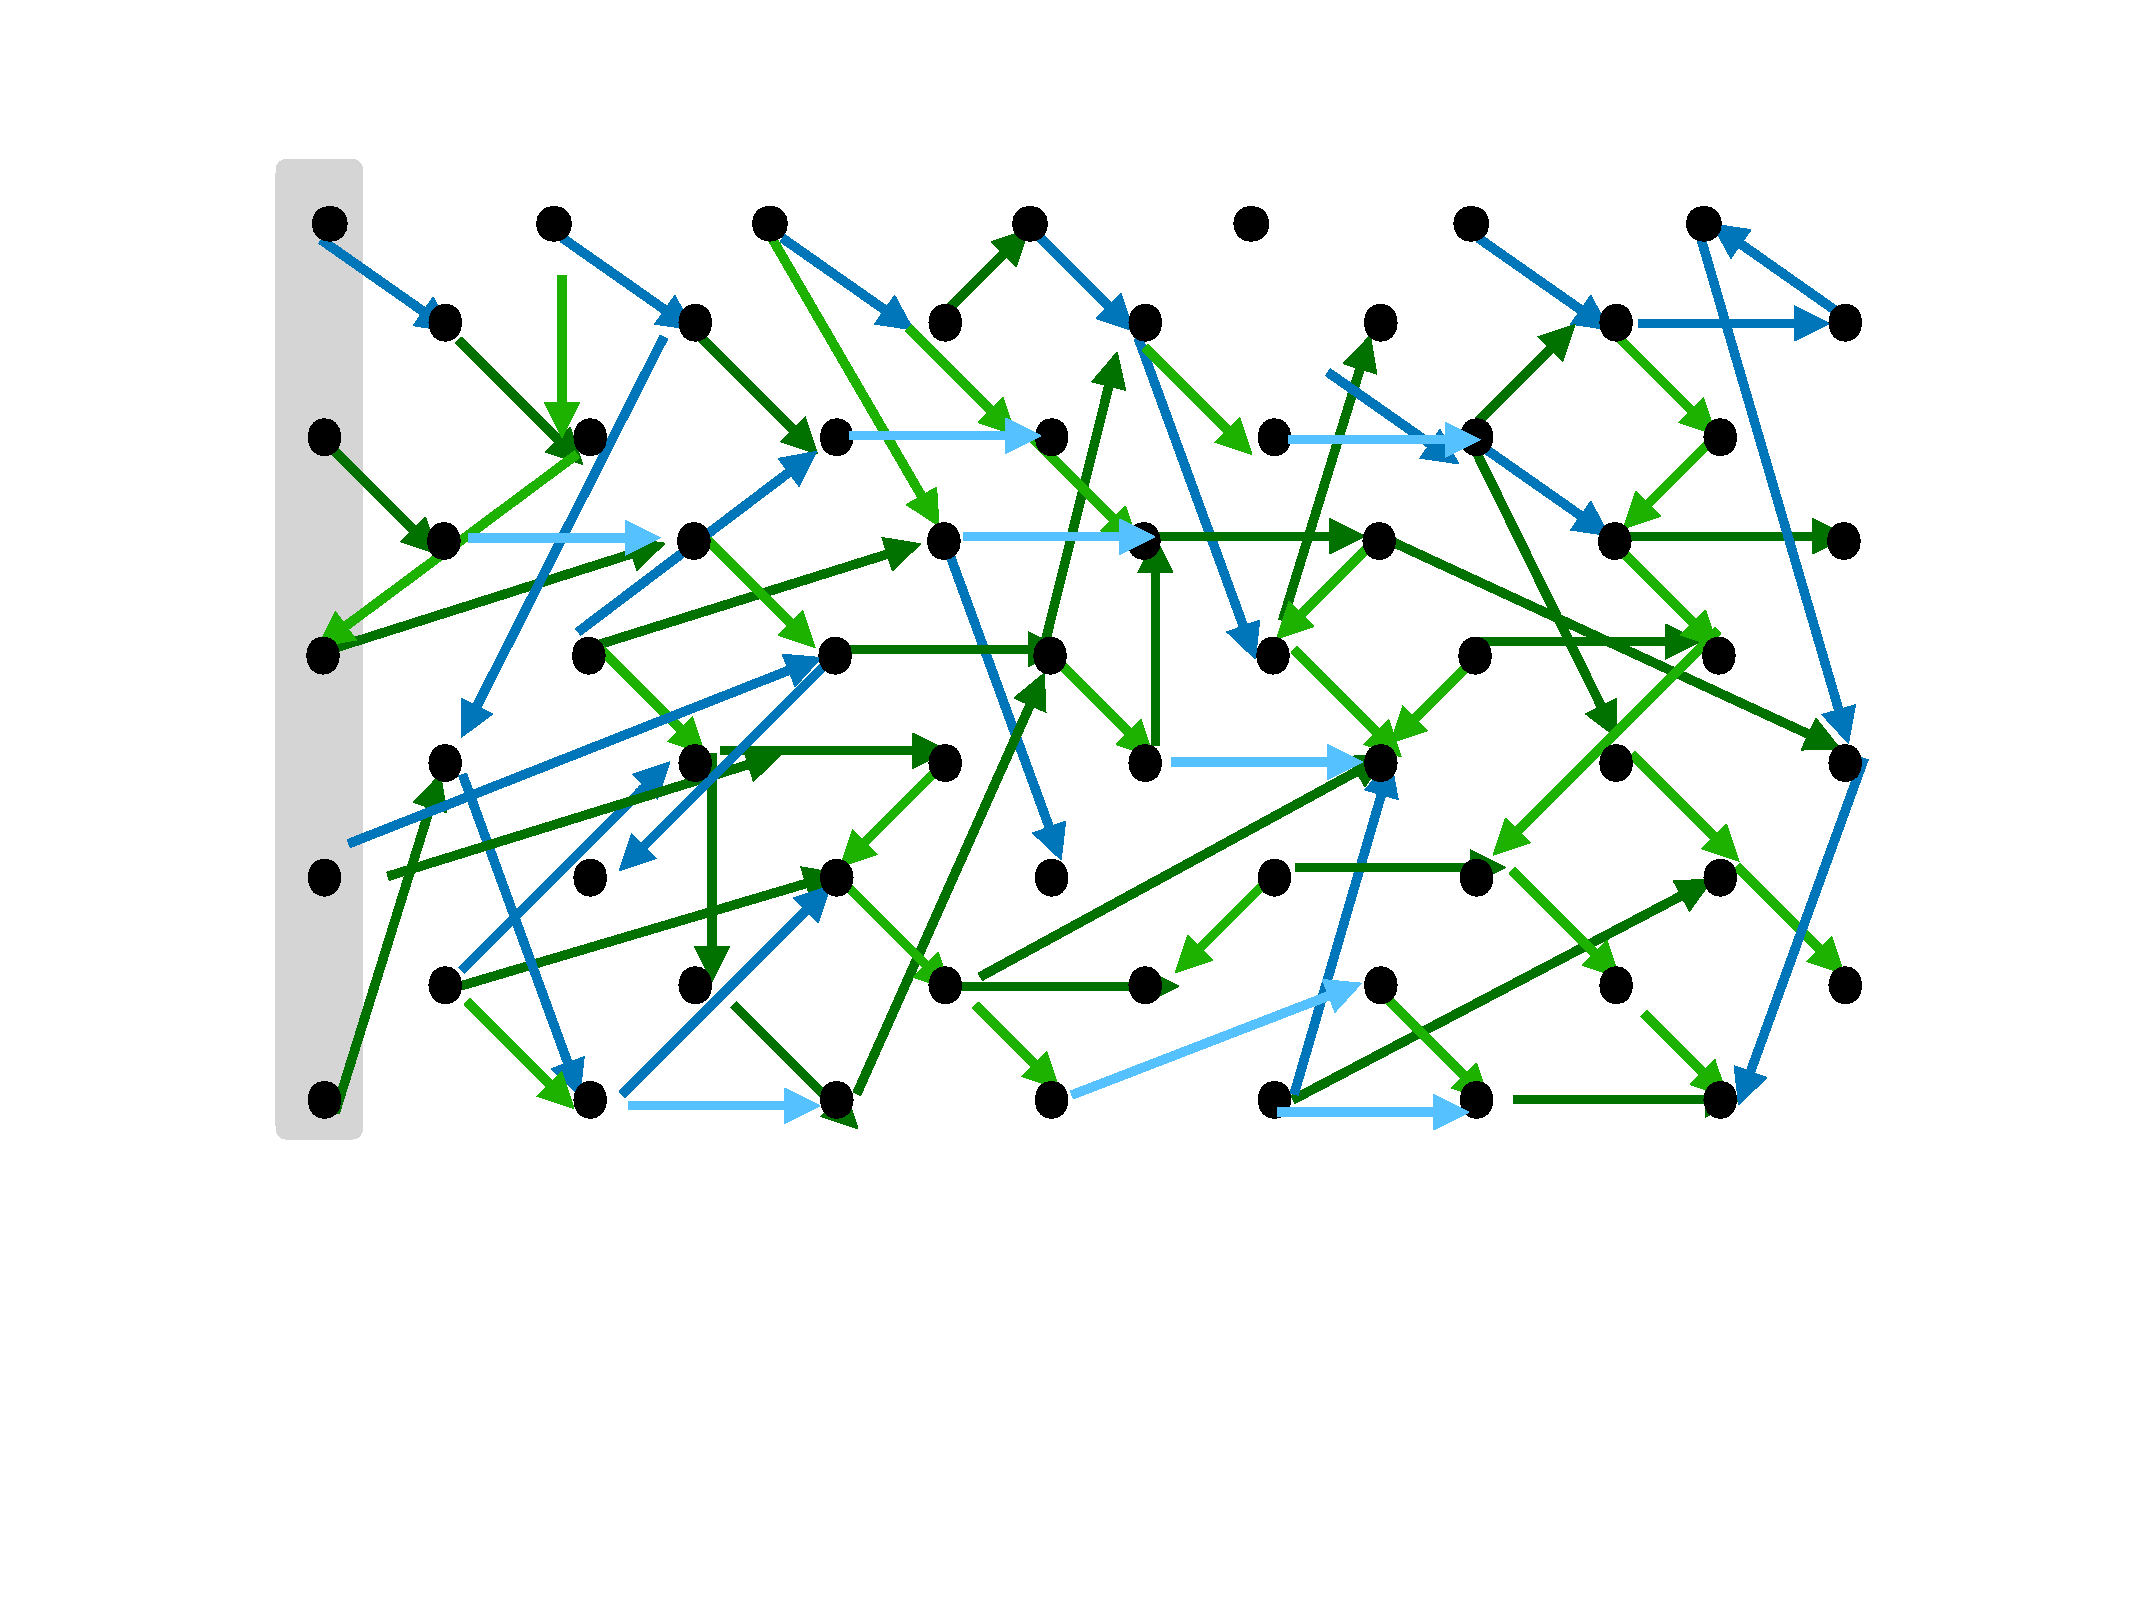
\includegraphics[width=\linewidth, trim=100  120 130 60,clip]{diagrams/neccSuff_yellow_A.pdf}
%\end{minipage}
% & \ \ \ & 
%\begin{minipage}{0.29\textwidth}
% 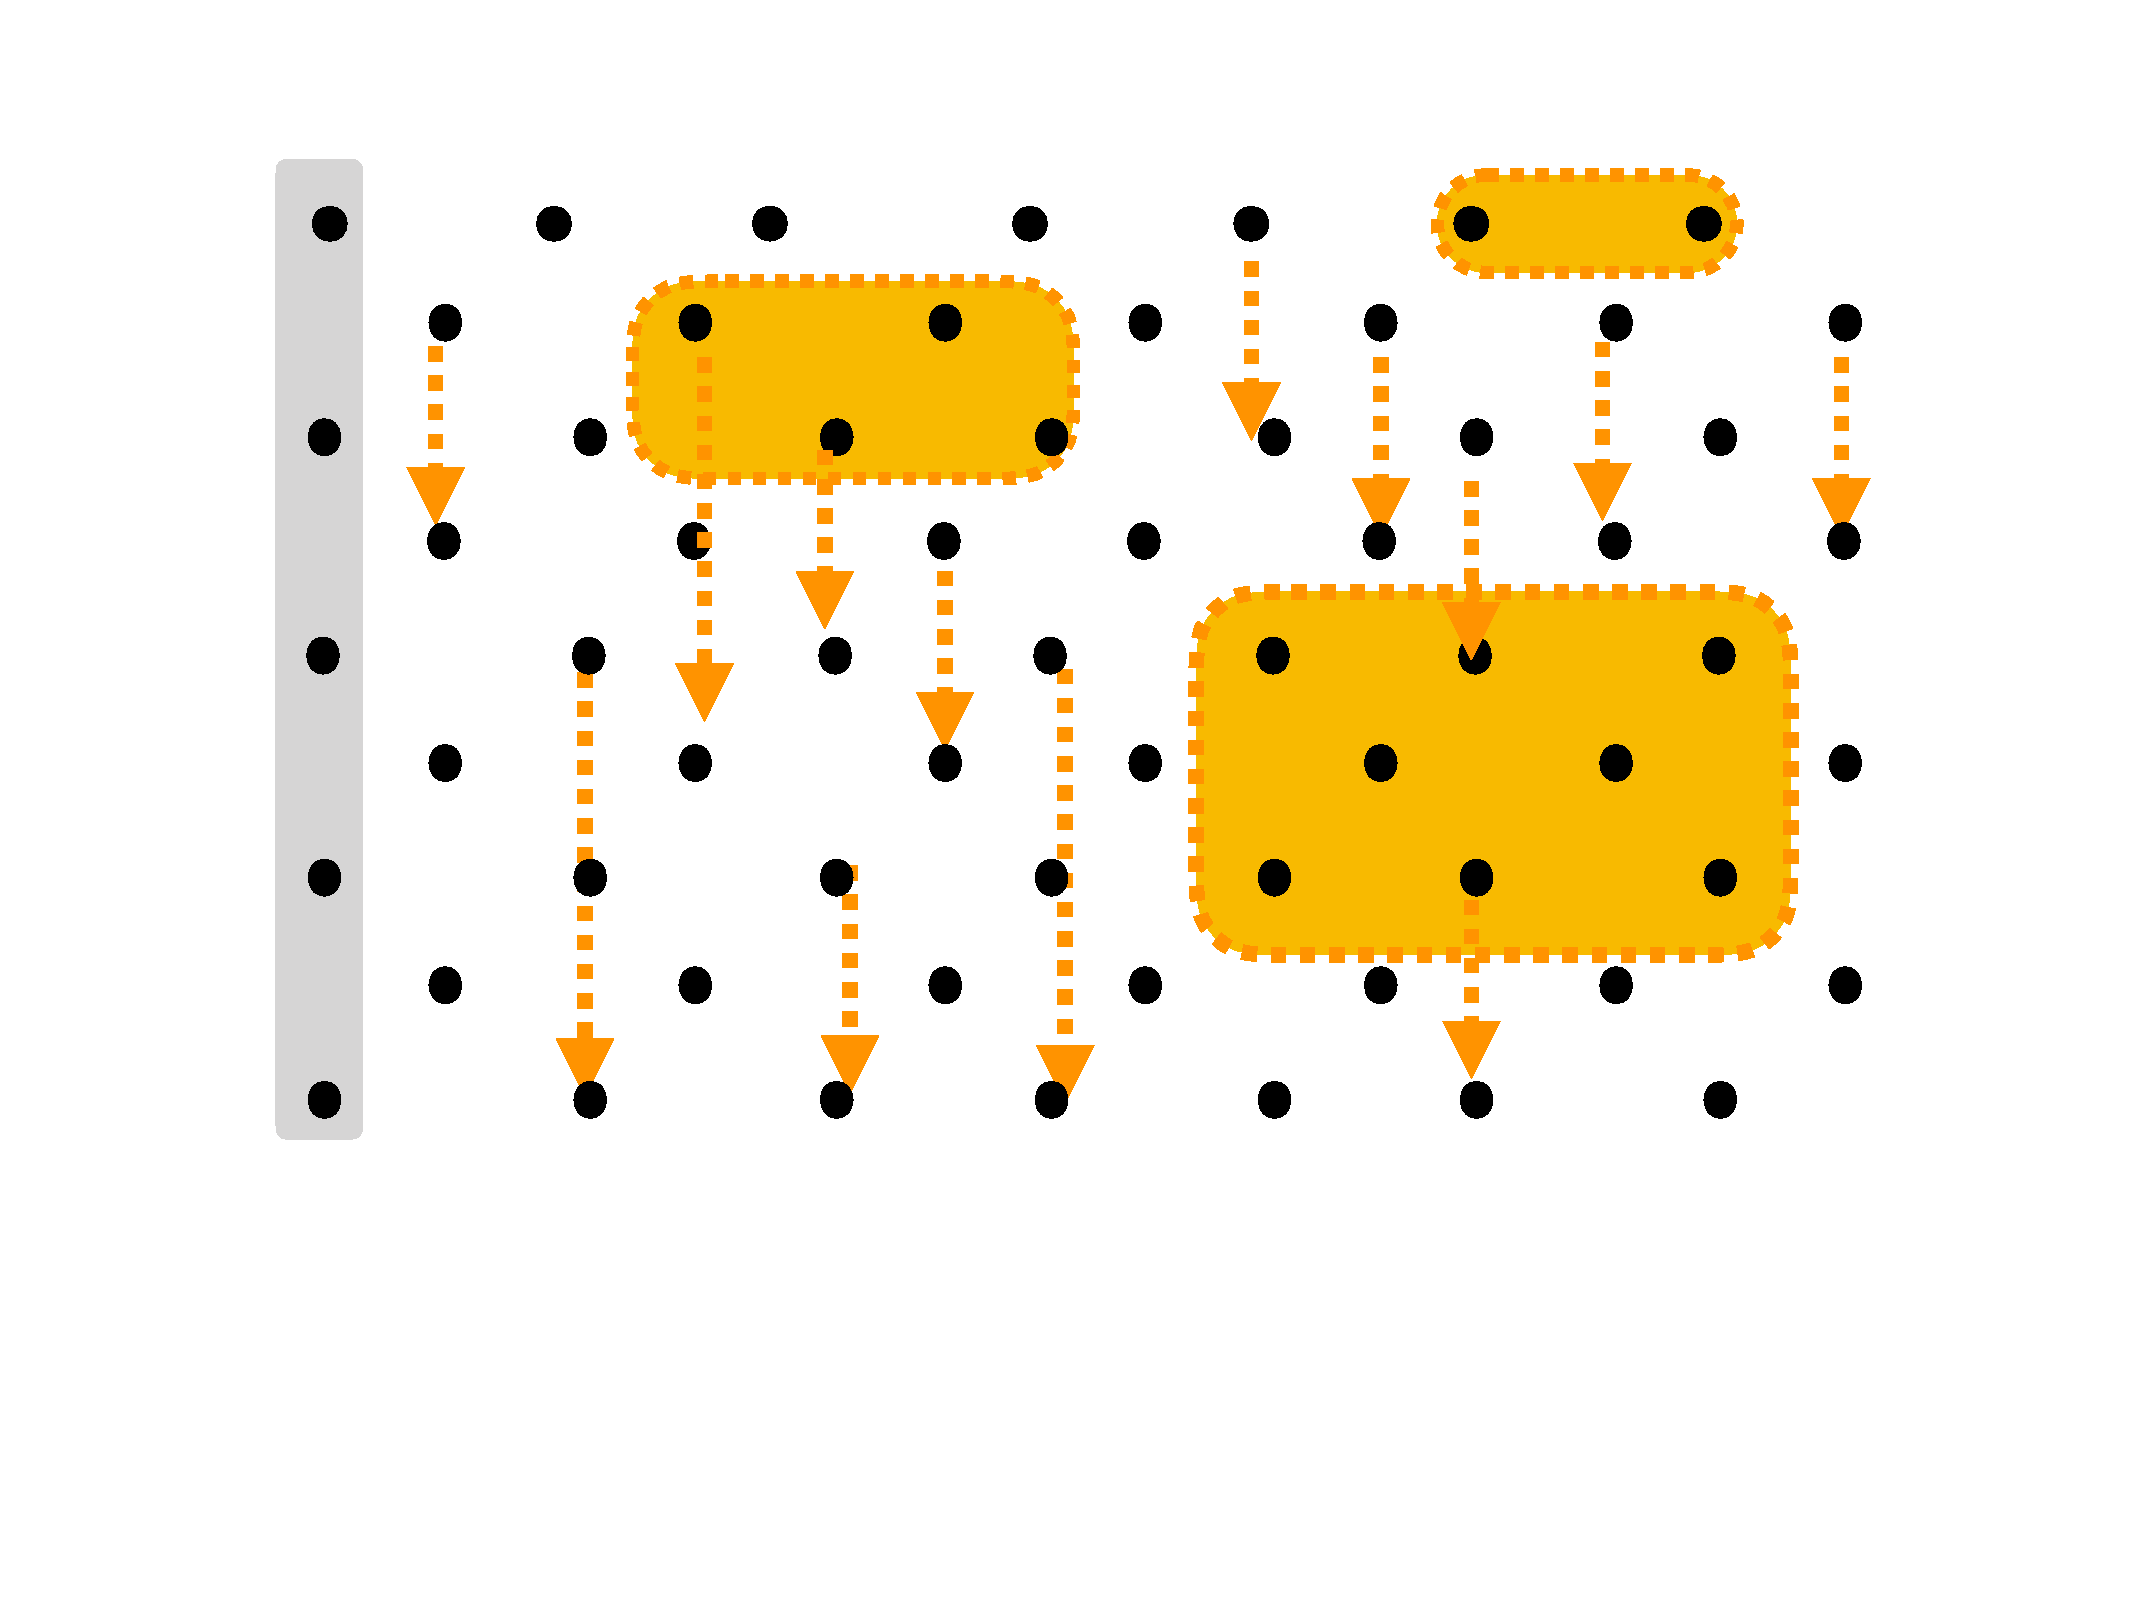
\includegraphics[width=\linewidth, trim=100  120 130 60,clip]{diagrams/neccSuff_yellow_B.pdf}
%\end{minipage}
% & \ \ \ &
%\begin{minipage}{0.29\textwidth}
% 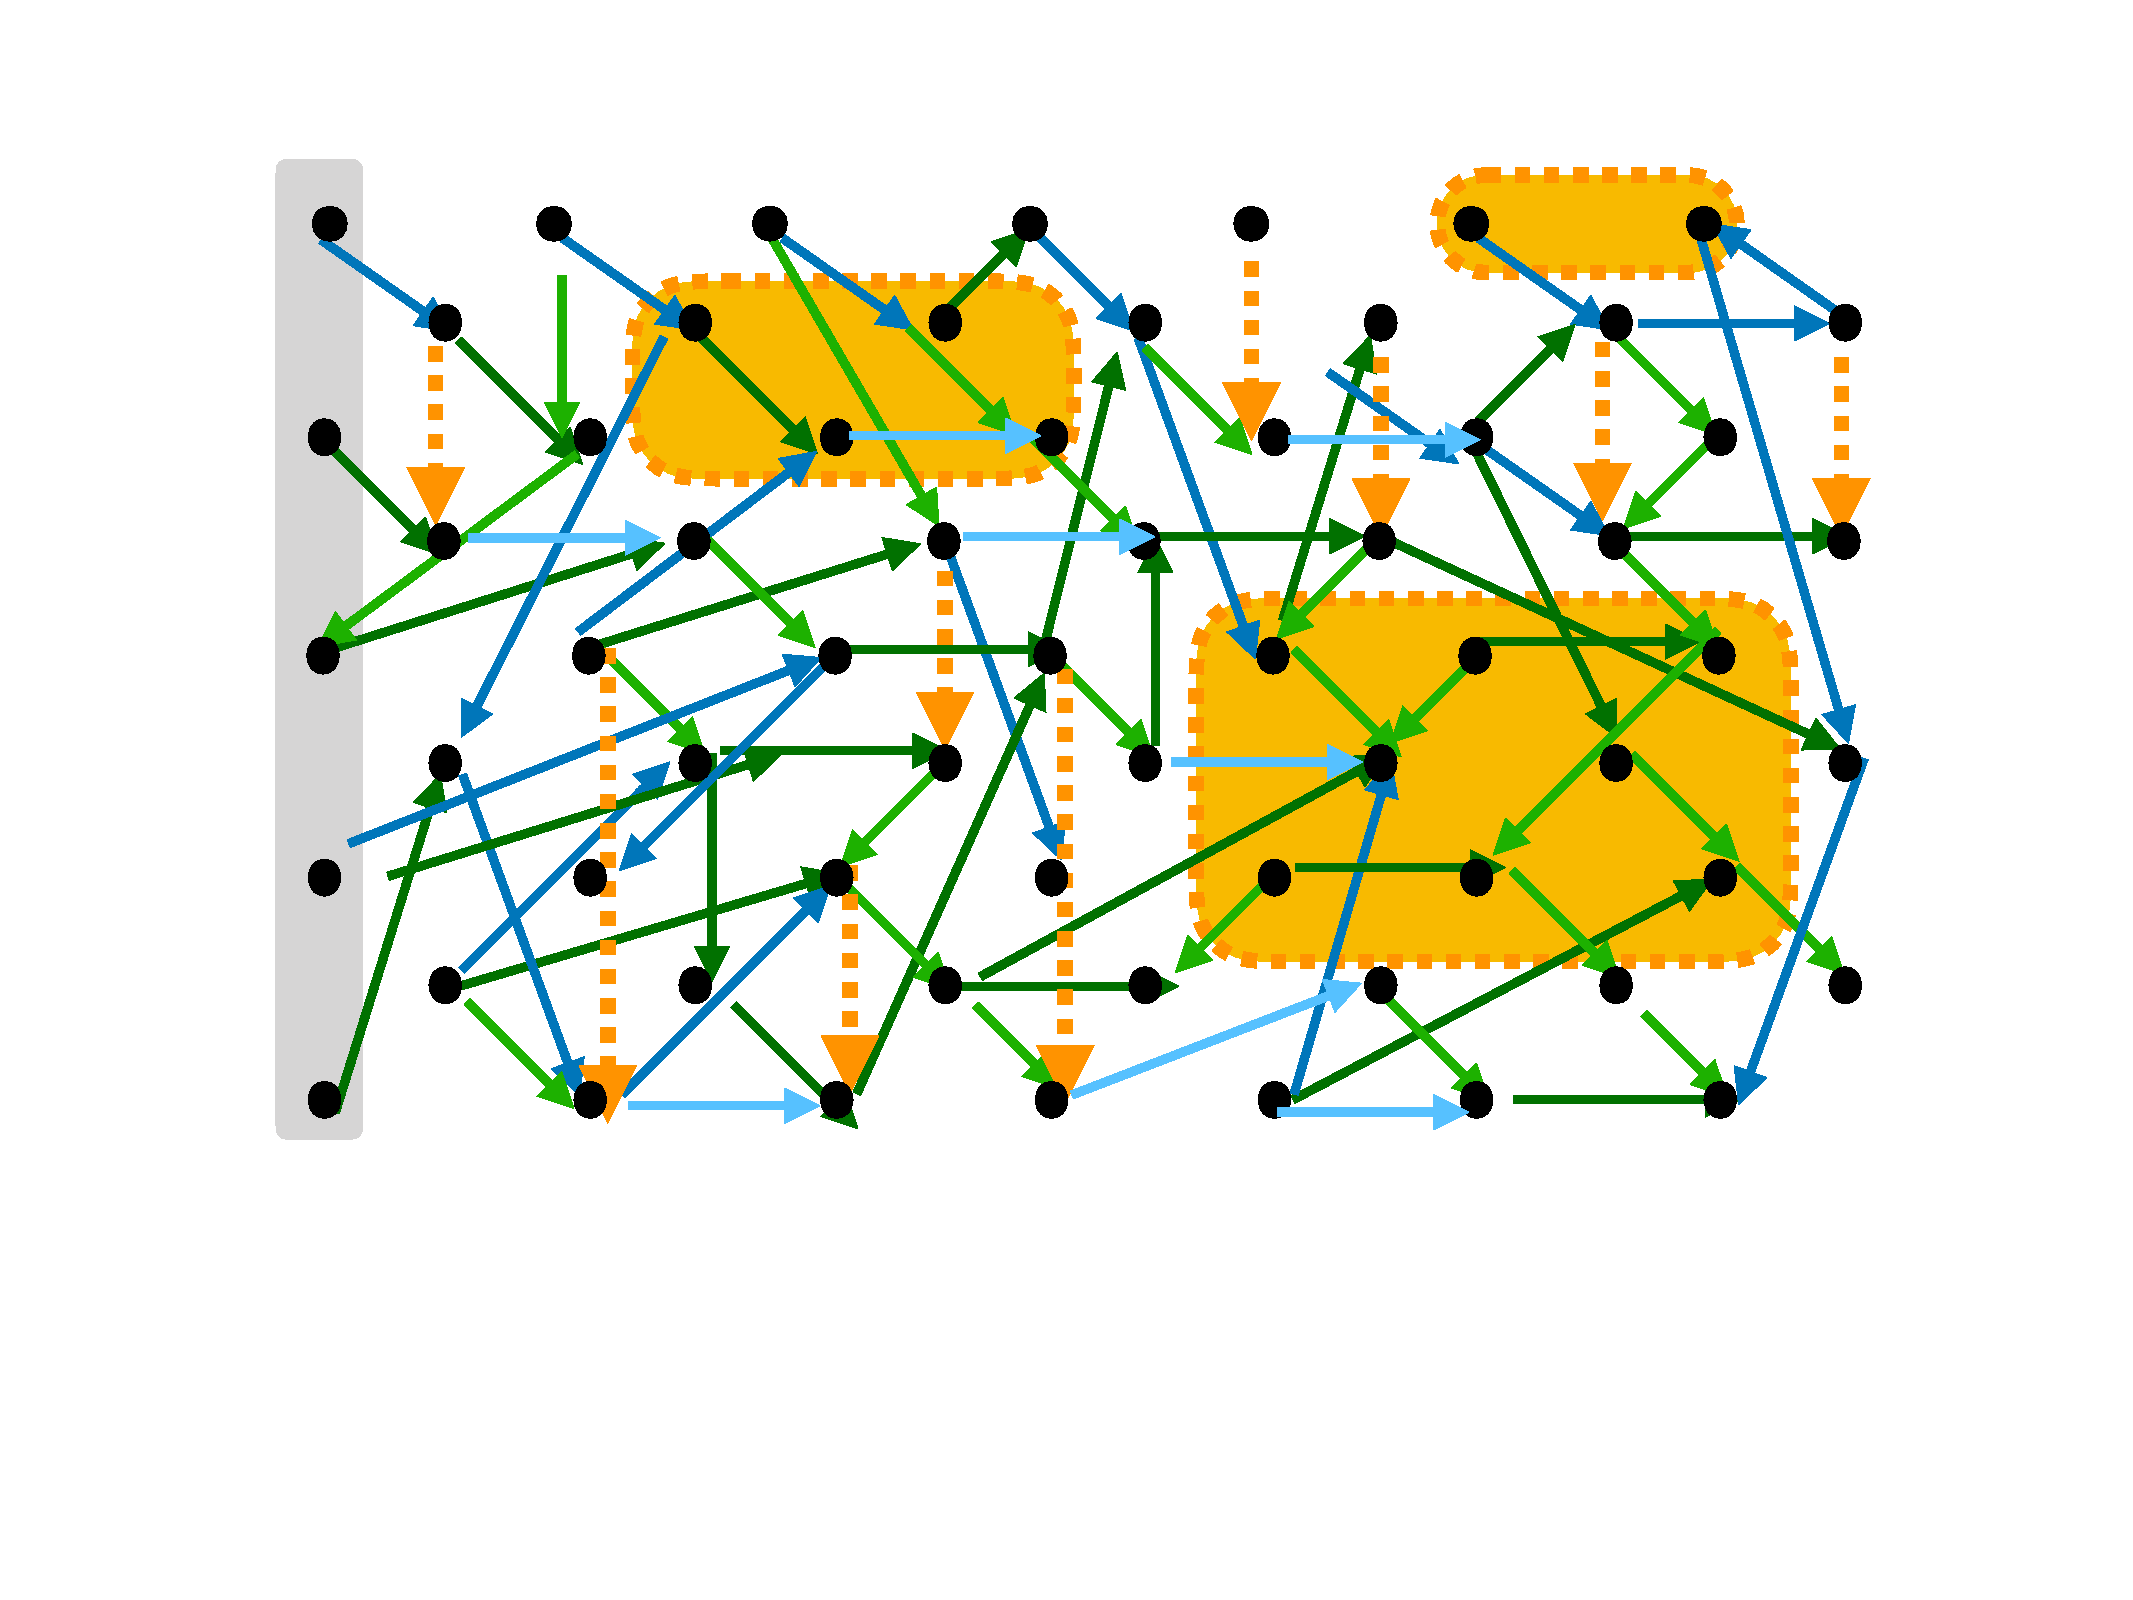
\includegraphics[width=\linewidth, trim=100  120 130 60,clip]{diagrams/neccSuffYellowAll.pdf}
% \end{minipage}
%\\
%(a) sufficient  spec.& & (b) necessary spec. & & (c) full, holistic spec.
%%\begin{minipage}{0.75\textwidth}
%%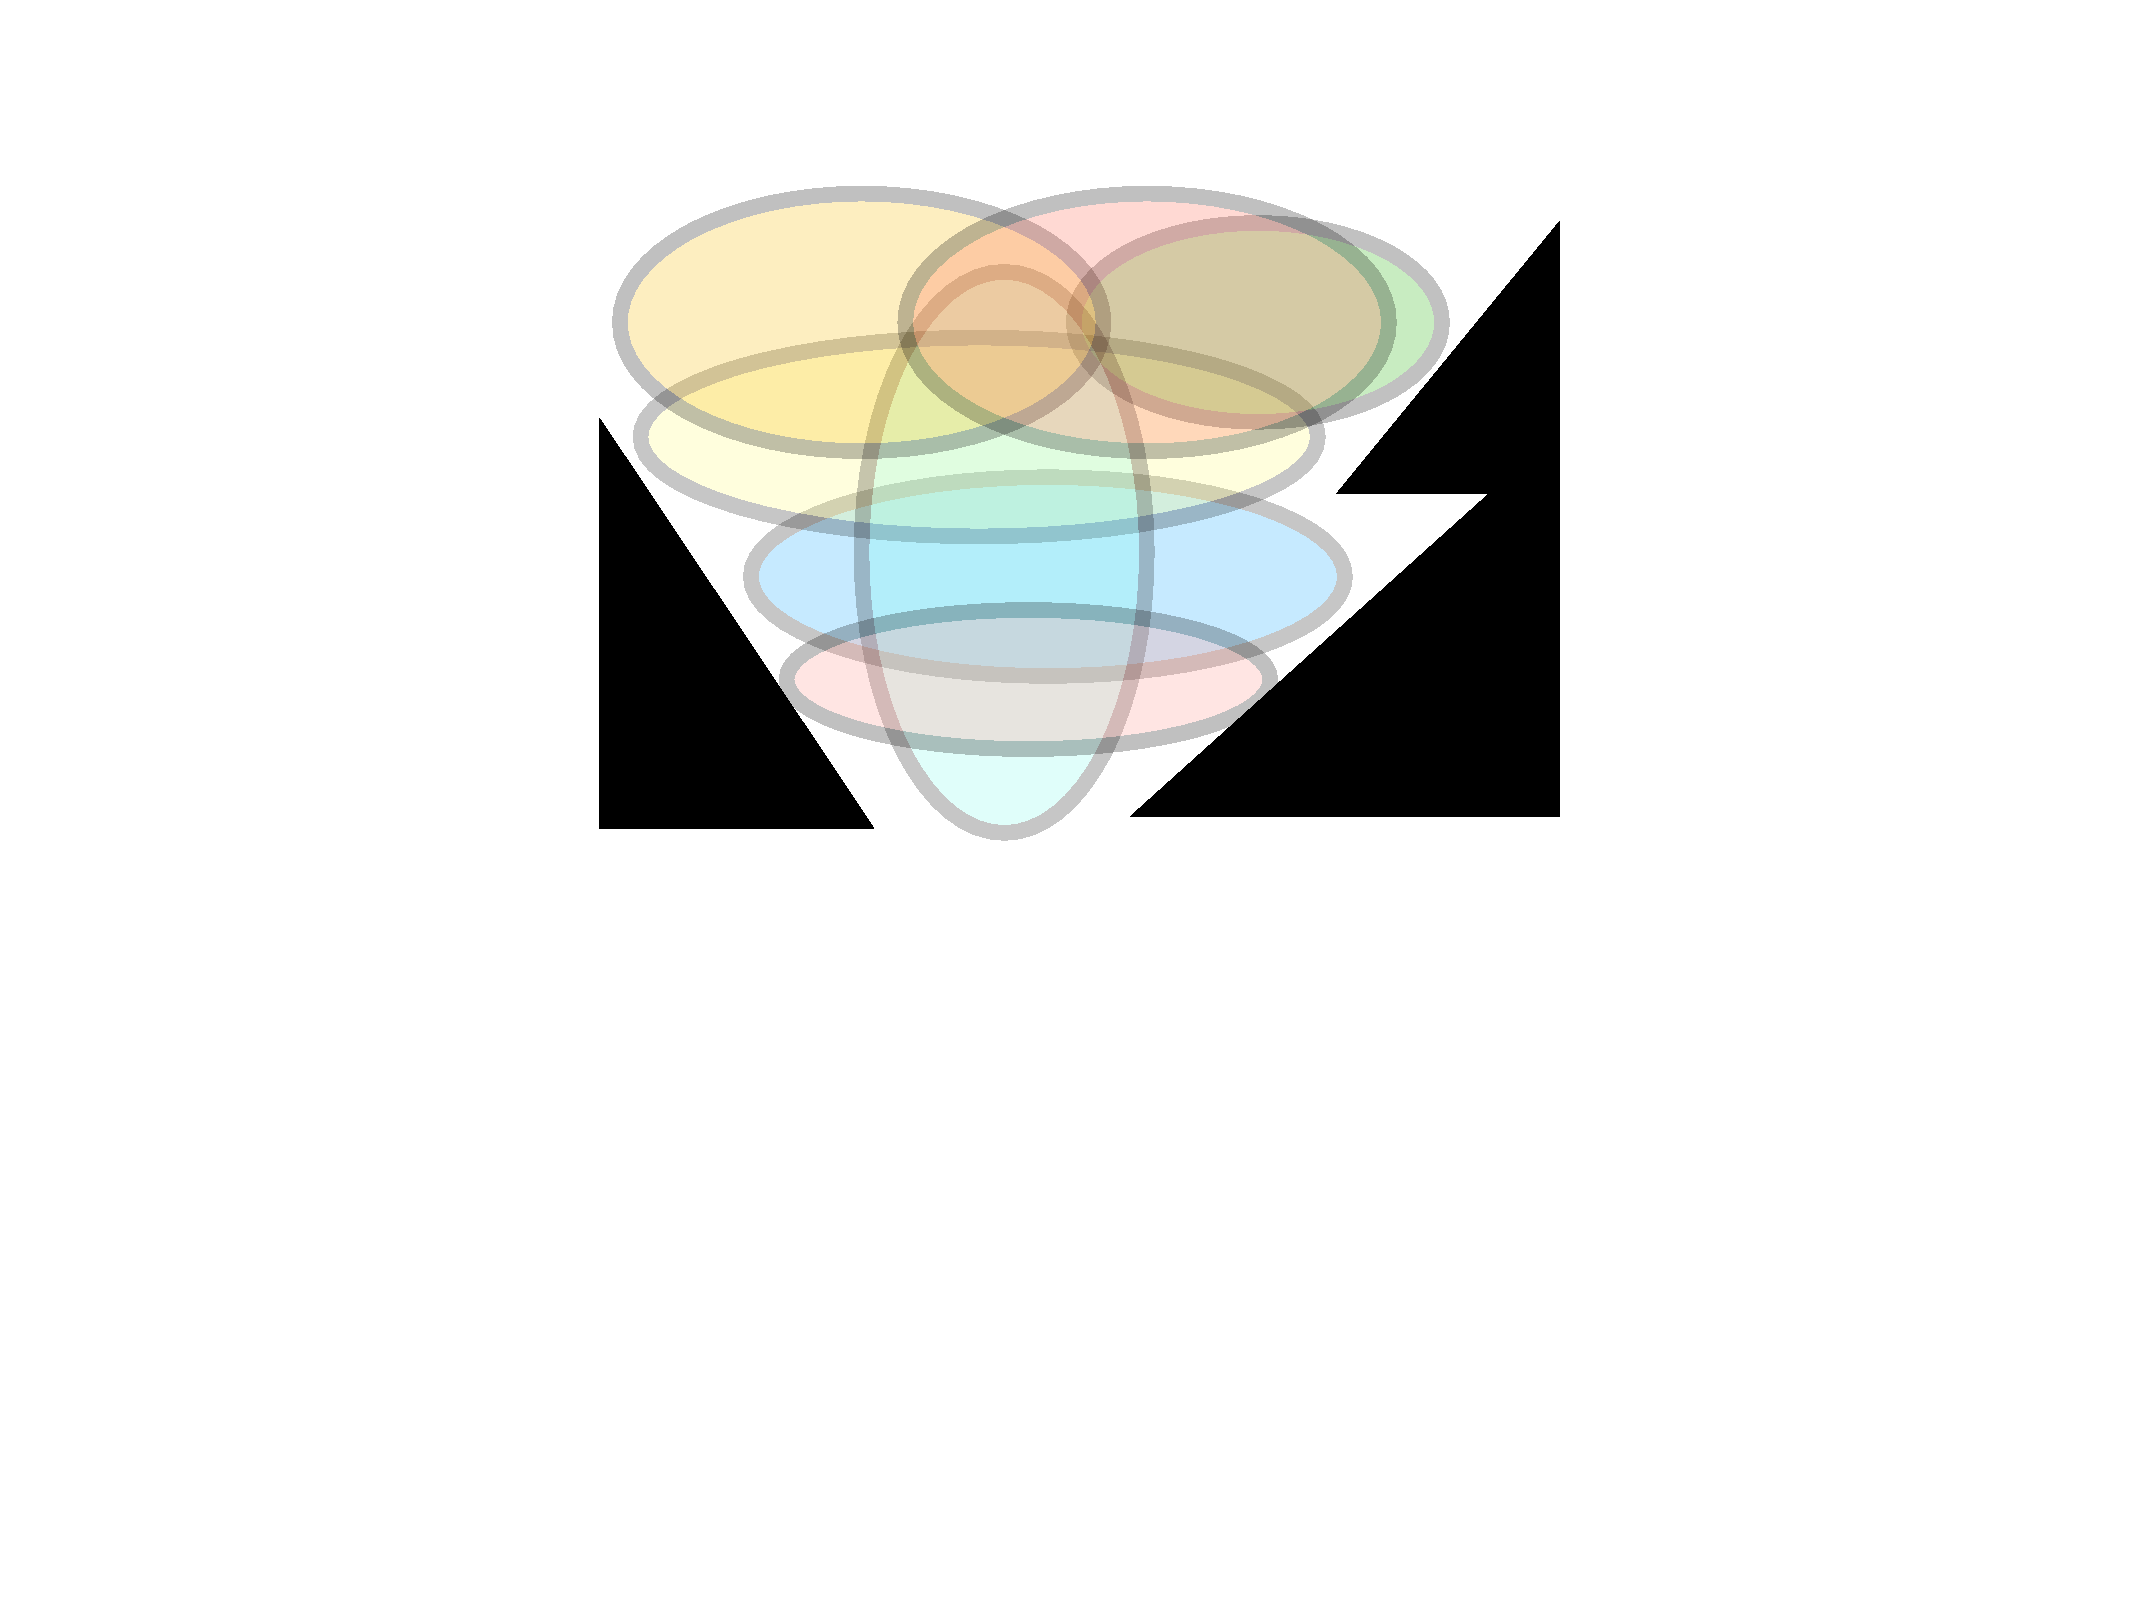
\includegraphics[width=\linewidth, trim=145  320 60 105,clip]{diagrams/NecAndSuff.pdf}
%%\end{minipage}
%%% y seems to eat up the bollom
%%% x eats space from left, if you increase it the diagram decreases from left
%%% w eats space from top, if you increase it the diagram decreases from top
%%%\includegraphics[page=3, width=\linewidth, trim=150  270 40 150, clip]{diagrams/snmallocf.pdf}
%%\sdcomment\sophia{I think we need to change the diagram so that it says small slab.}
%%\end{minipage}
% \end{tabular}
%  \vspace*{-2.5mm}
%  \caption{Sufficient Conditions, Necessary Conditions, and Full Specifications}
% \label{fig:NecessaryAndSuff}
% \end{figure}
 
 

 
 
 We propose that  necessary conditions should be stated
 explicitly. Specifications should be \emph{holistic}, in the sense
 that they describe the  overall behaviour of a component: not only the
 behaviour of each individual function, but also limitations on the
 behaviour that emerges from combinations of functions.
%
%Holistic specifications must therefore address sufficient as well as necessary conditions, as  
%depicted in part (c)    in Fig. \ref{fig:NecessaryAndSuff}.
%When a component \sd{satisfies its holistic specification},
%% used to say "has been specified holistically" but this is not sufficient
%then \sd{the states  in the yellow boxes and the 
%behaviours
%represented  by the yellow arrows} cannot occur, even when the
%component interacts with other software of unknown provenance.
%(In Section \ref{sect:discussion} we argue why necessary conditions are more than the complement of
%sufficient conditions.)
%
%% %
%%  \begin{figure}[htb]
%%  \begin{tabular}{clclc}
%% \begin{minipage}{0.29\textwidth}
%%  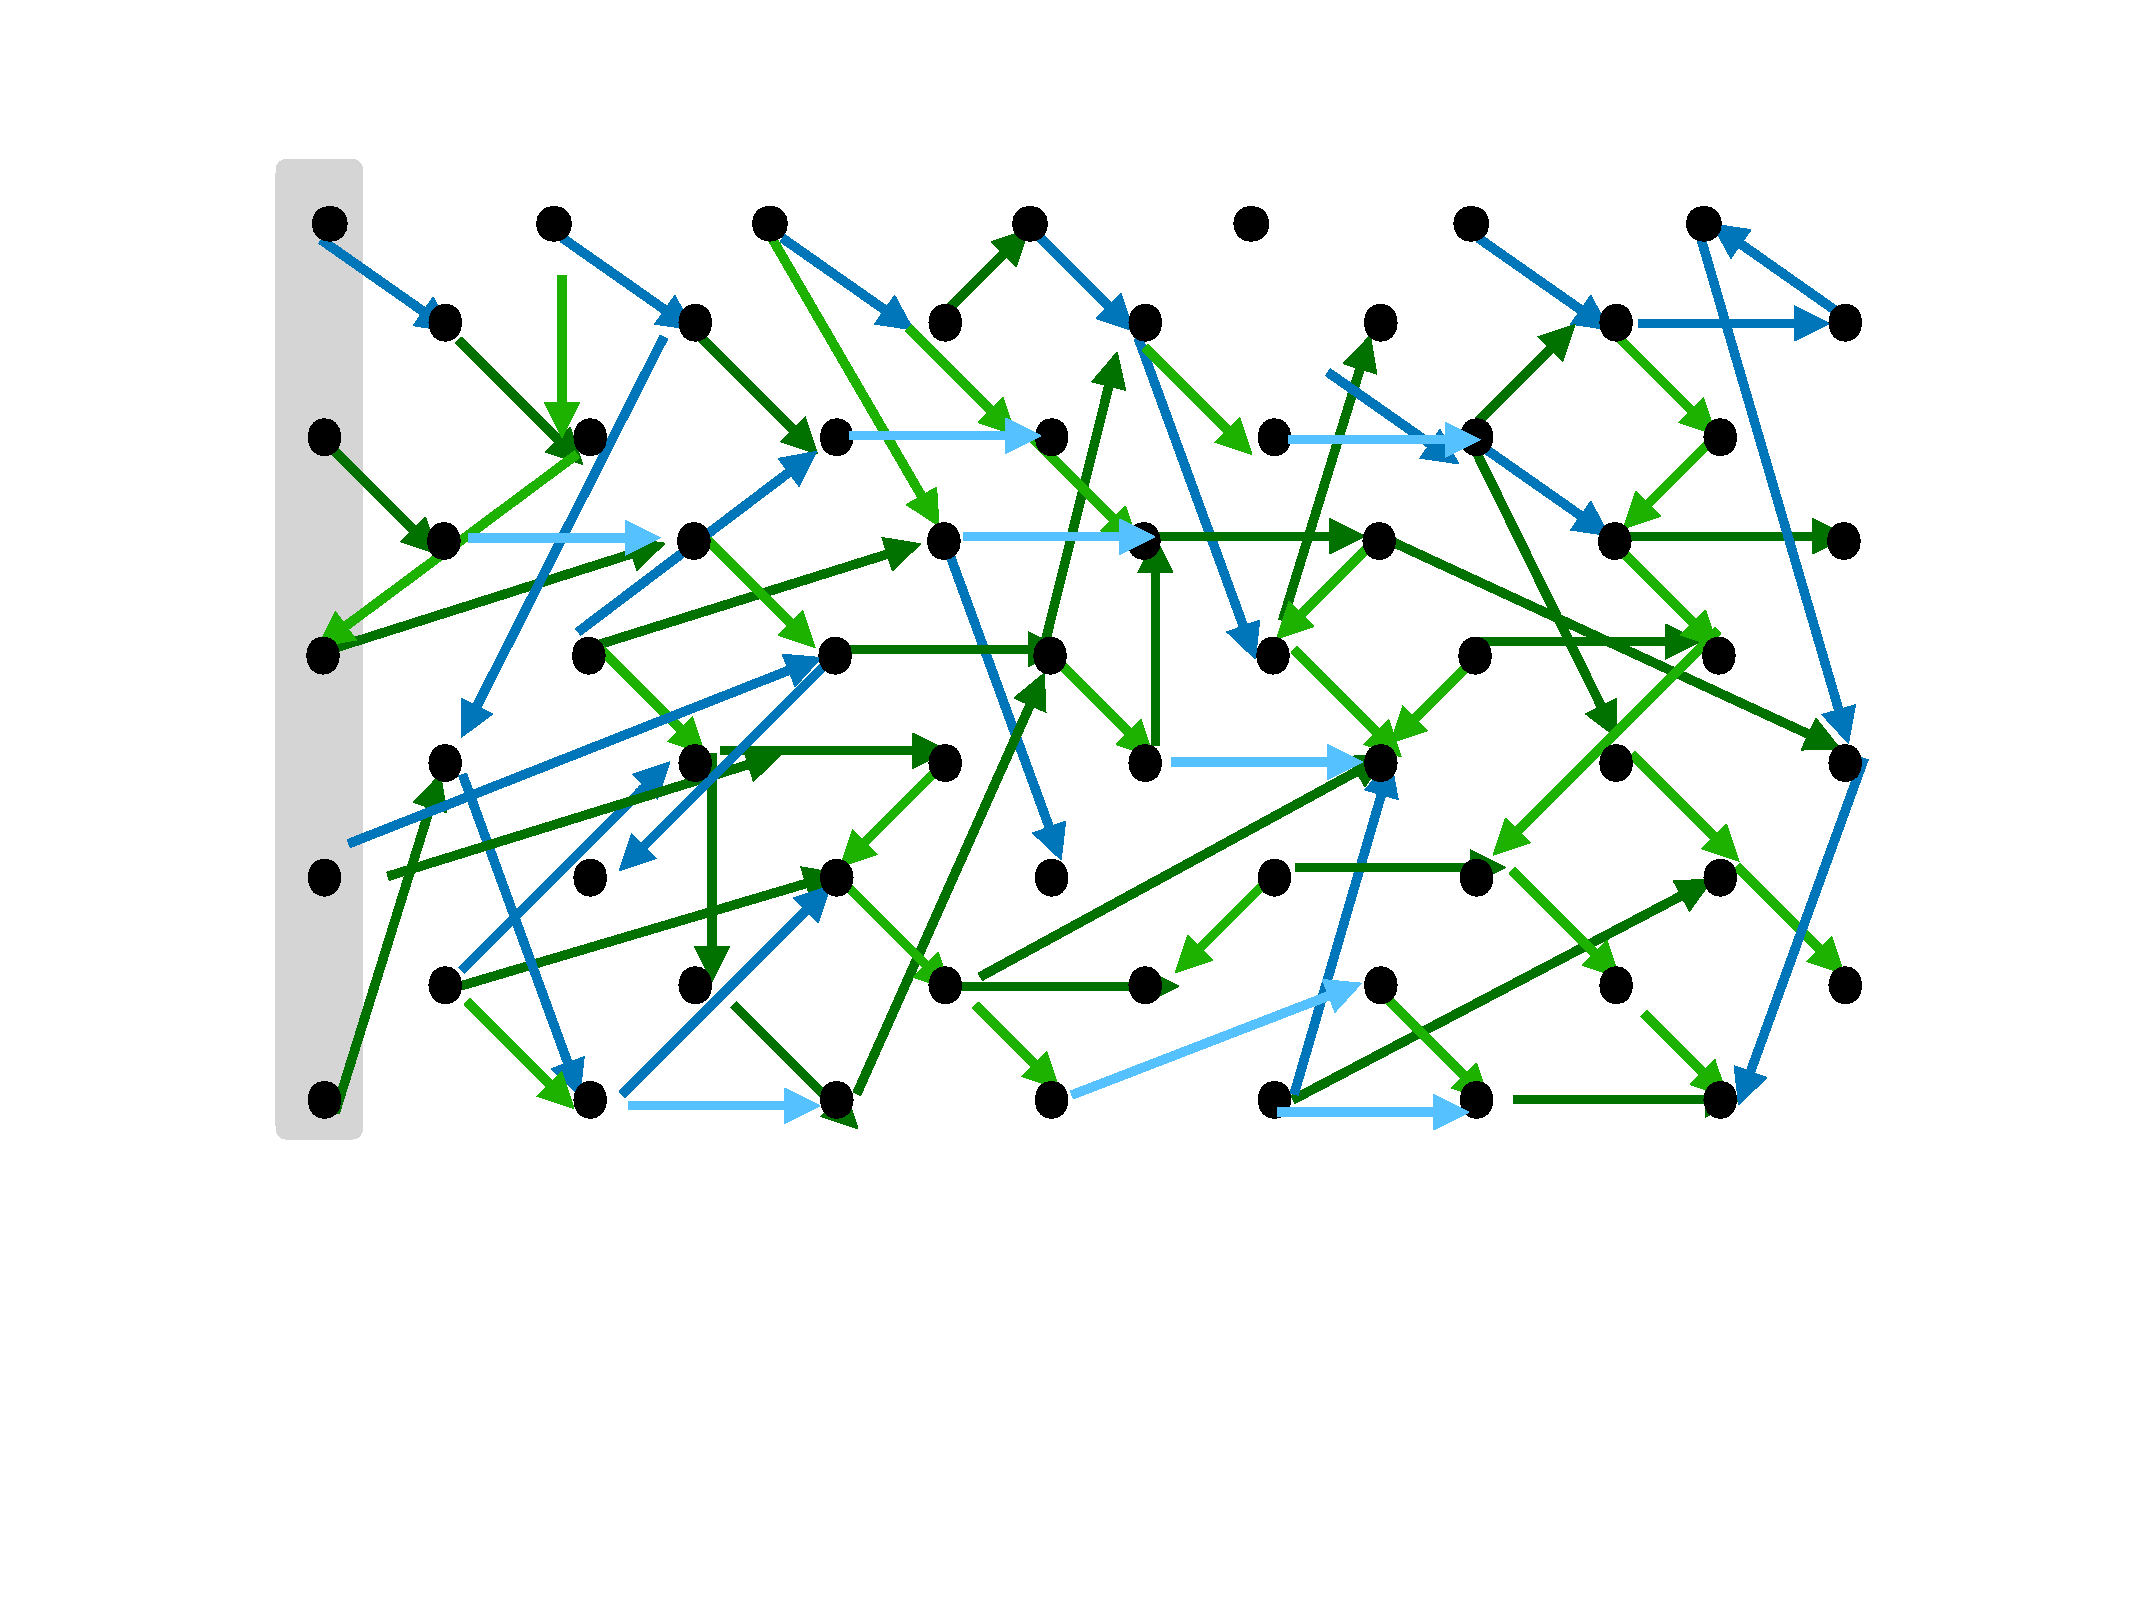
\includegraphics[width=\linewidth, trim=100  120 130 60,clip]{diagrams/neccSuff_yellow_A.pdf}
%% \end{minipage}
%%  & \ \ \ & 
%% \begin{minipage}{0.29\textwidth}
%%  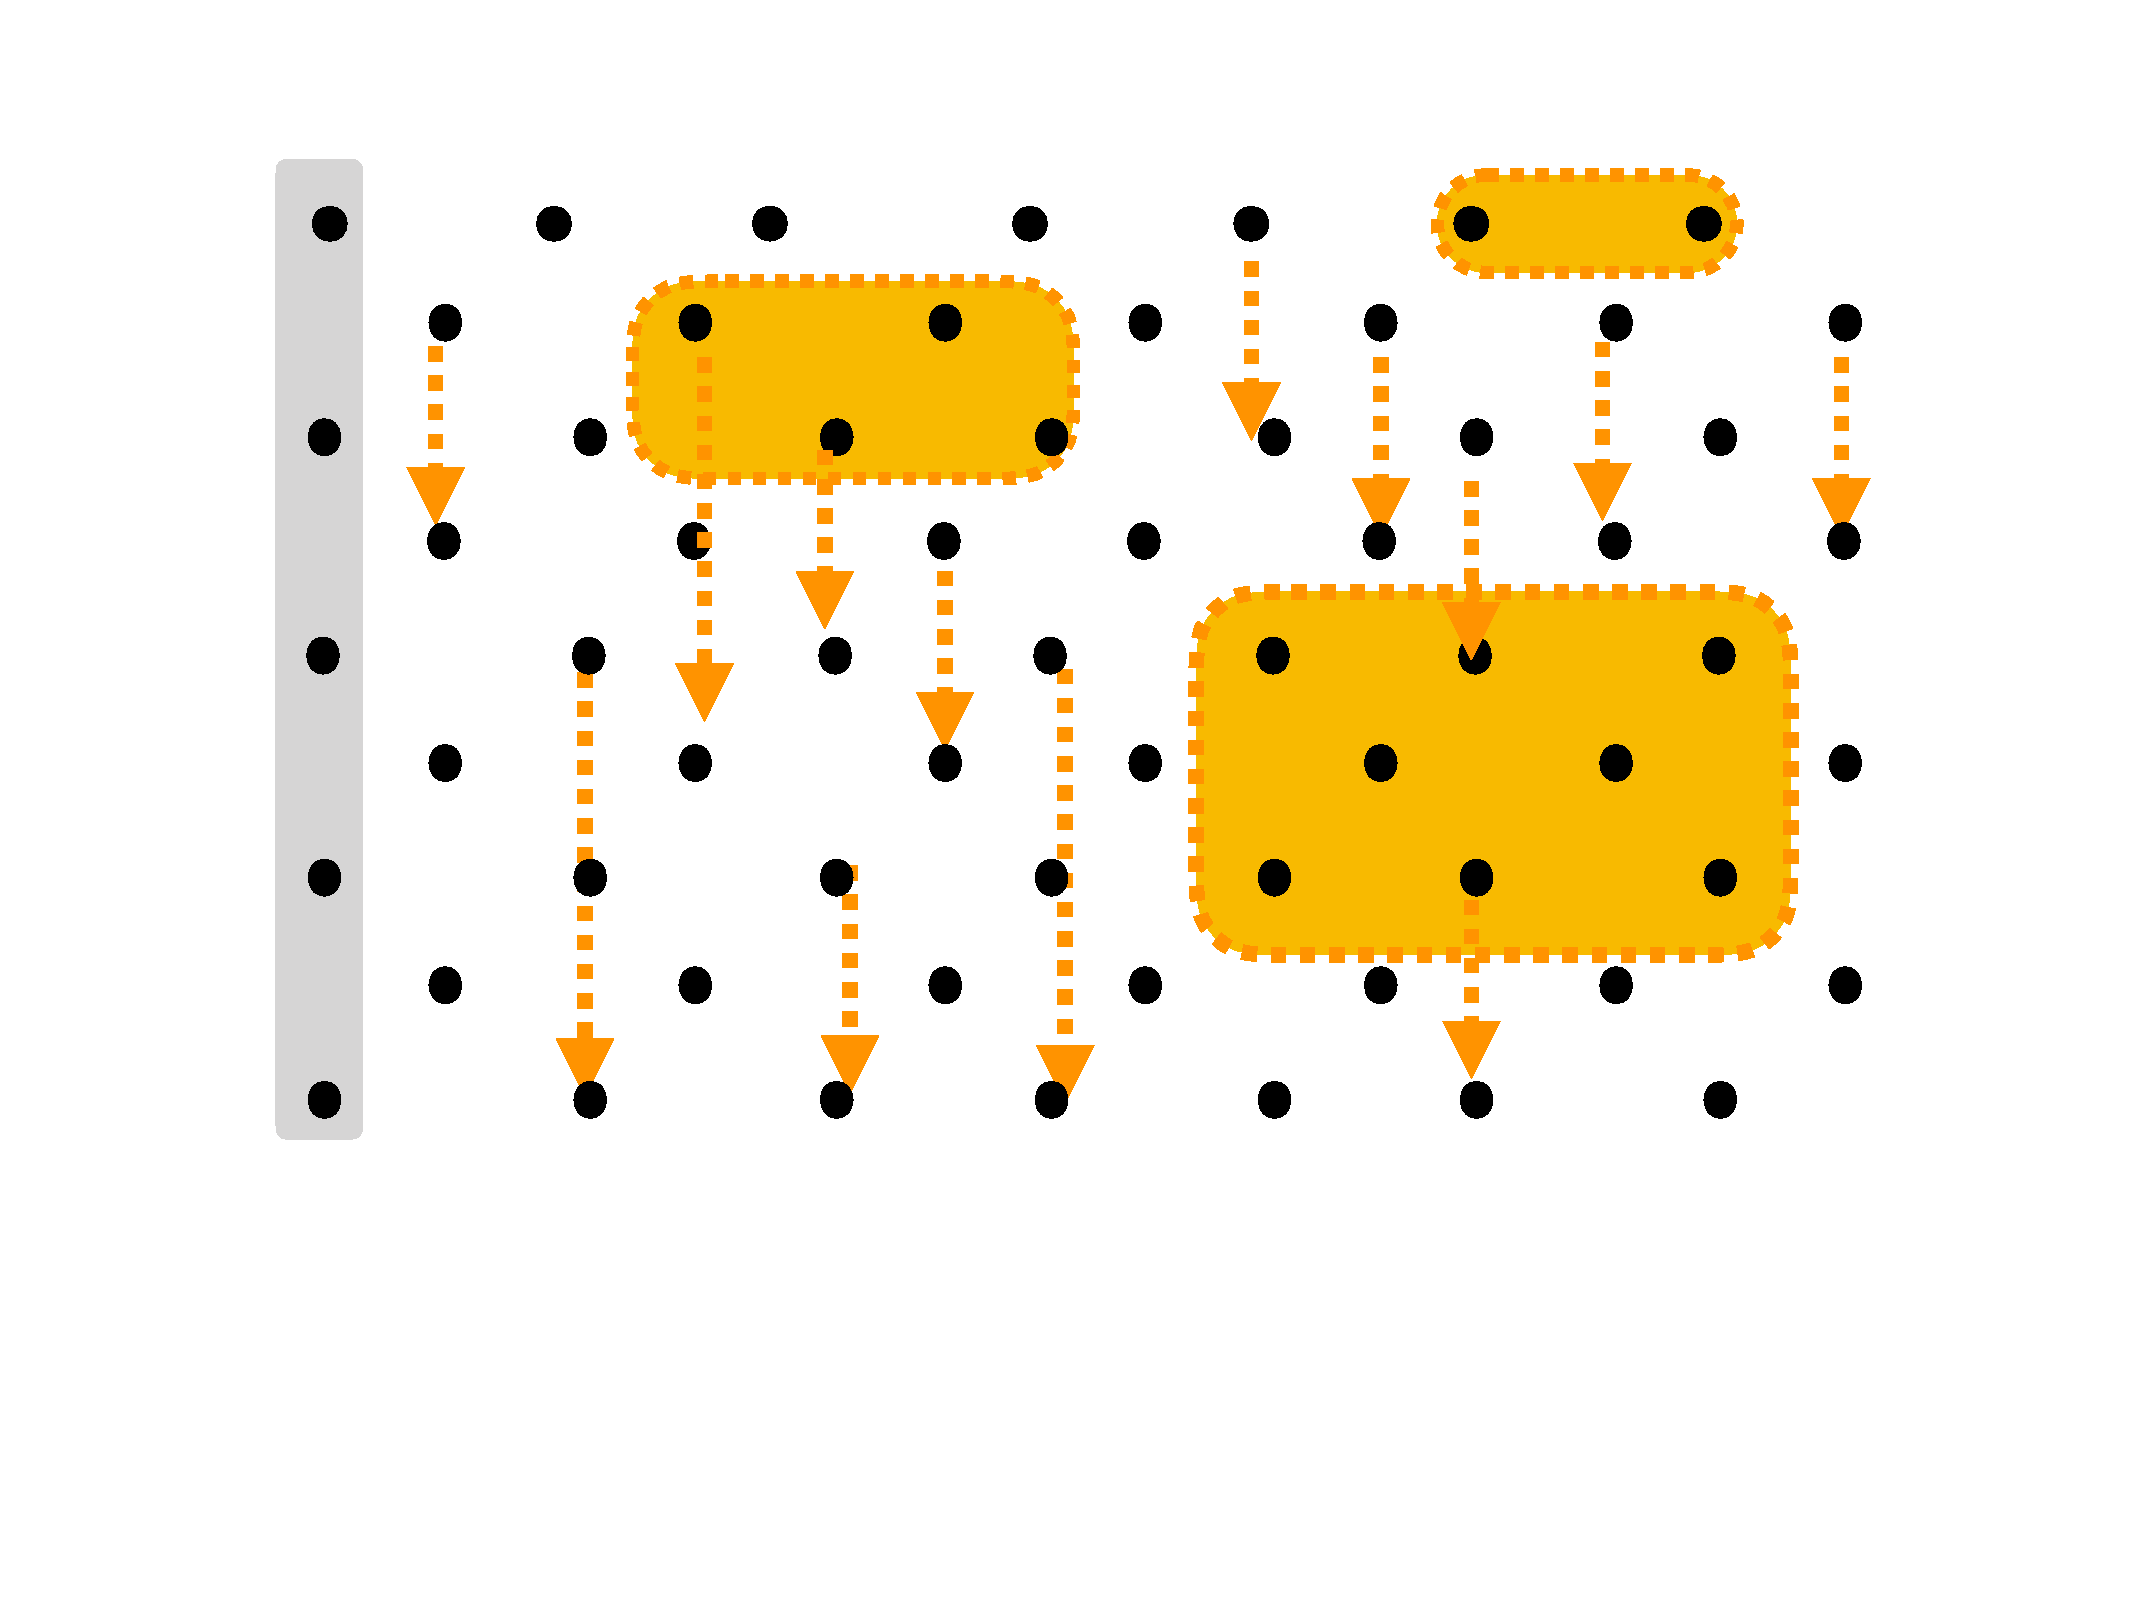
\includegraphics[width=\linewidth, trim=100  120 130 60,clip]{diagrams/neccSuff_yellow_B.pdf}
%% \end{minipage}
%%  & \ \ \ &
%% \begin{minipage}{0.29\textwidth}
%%  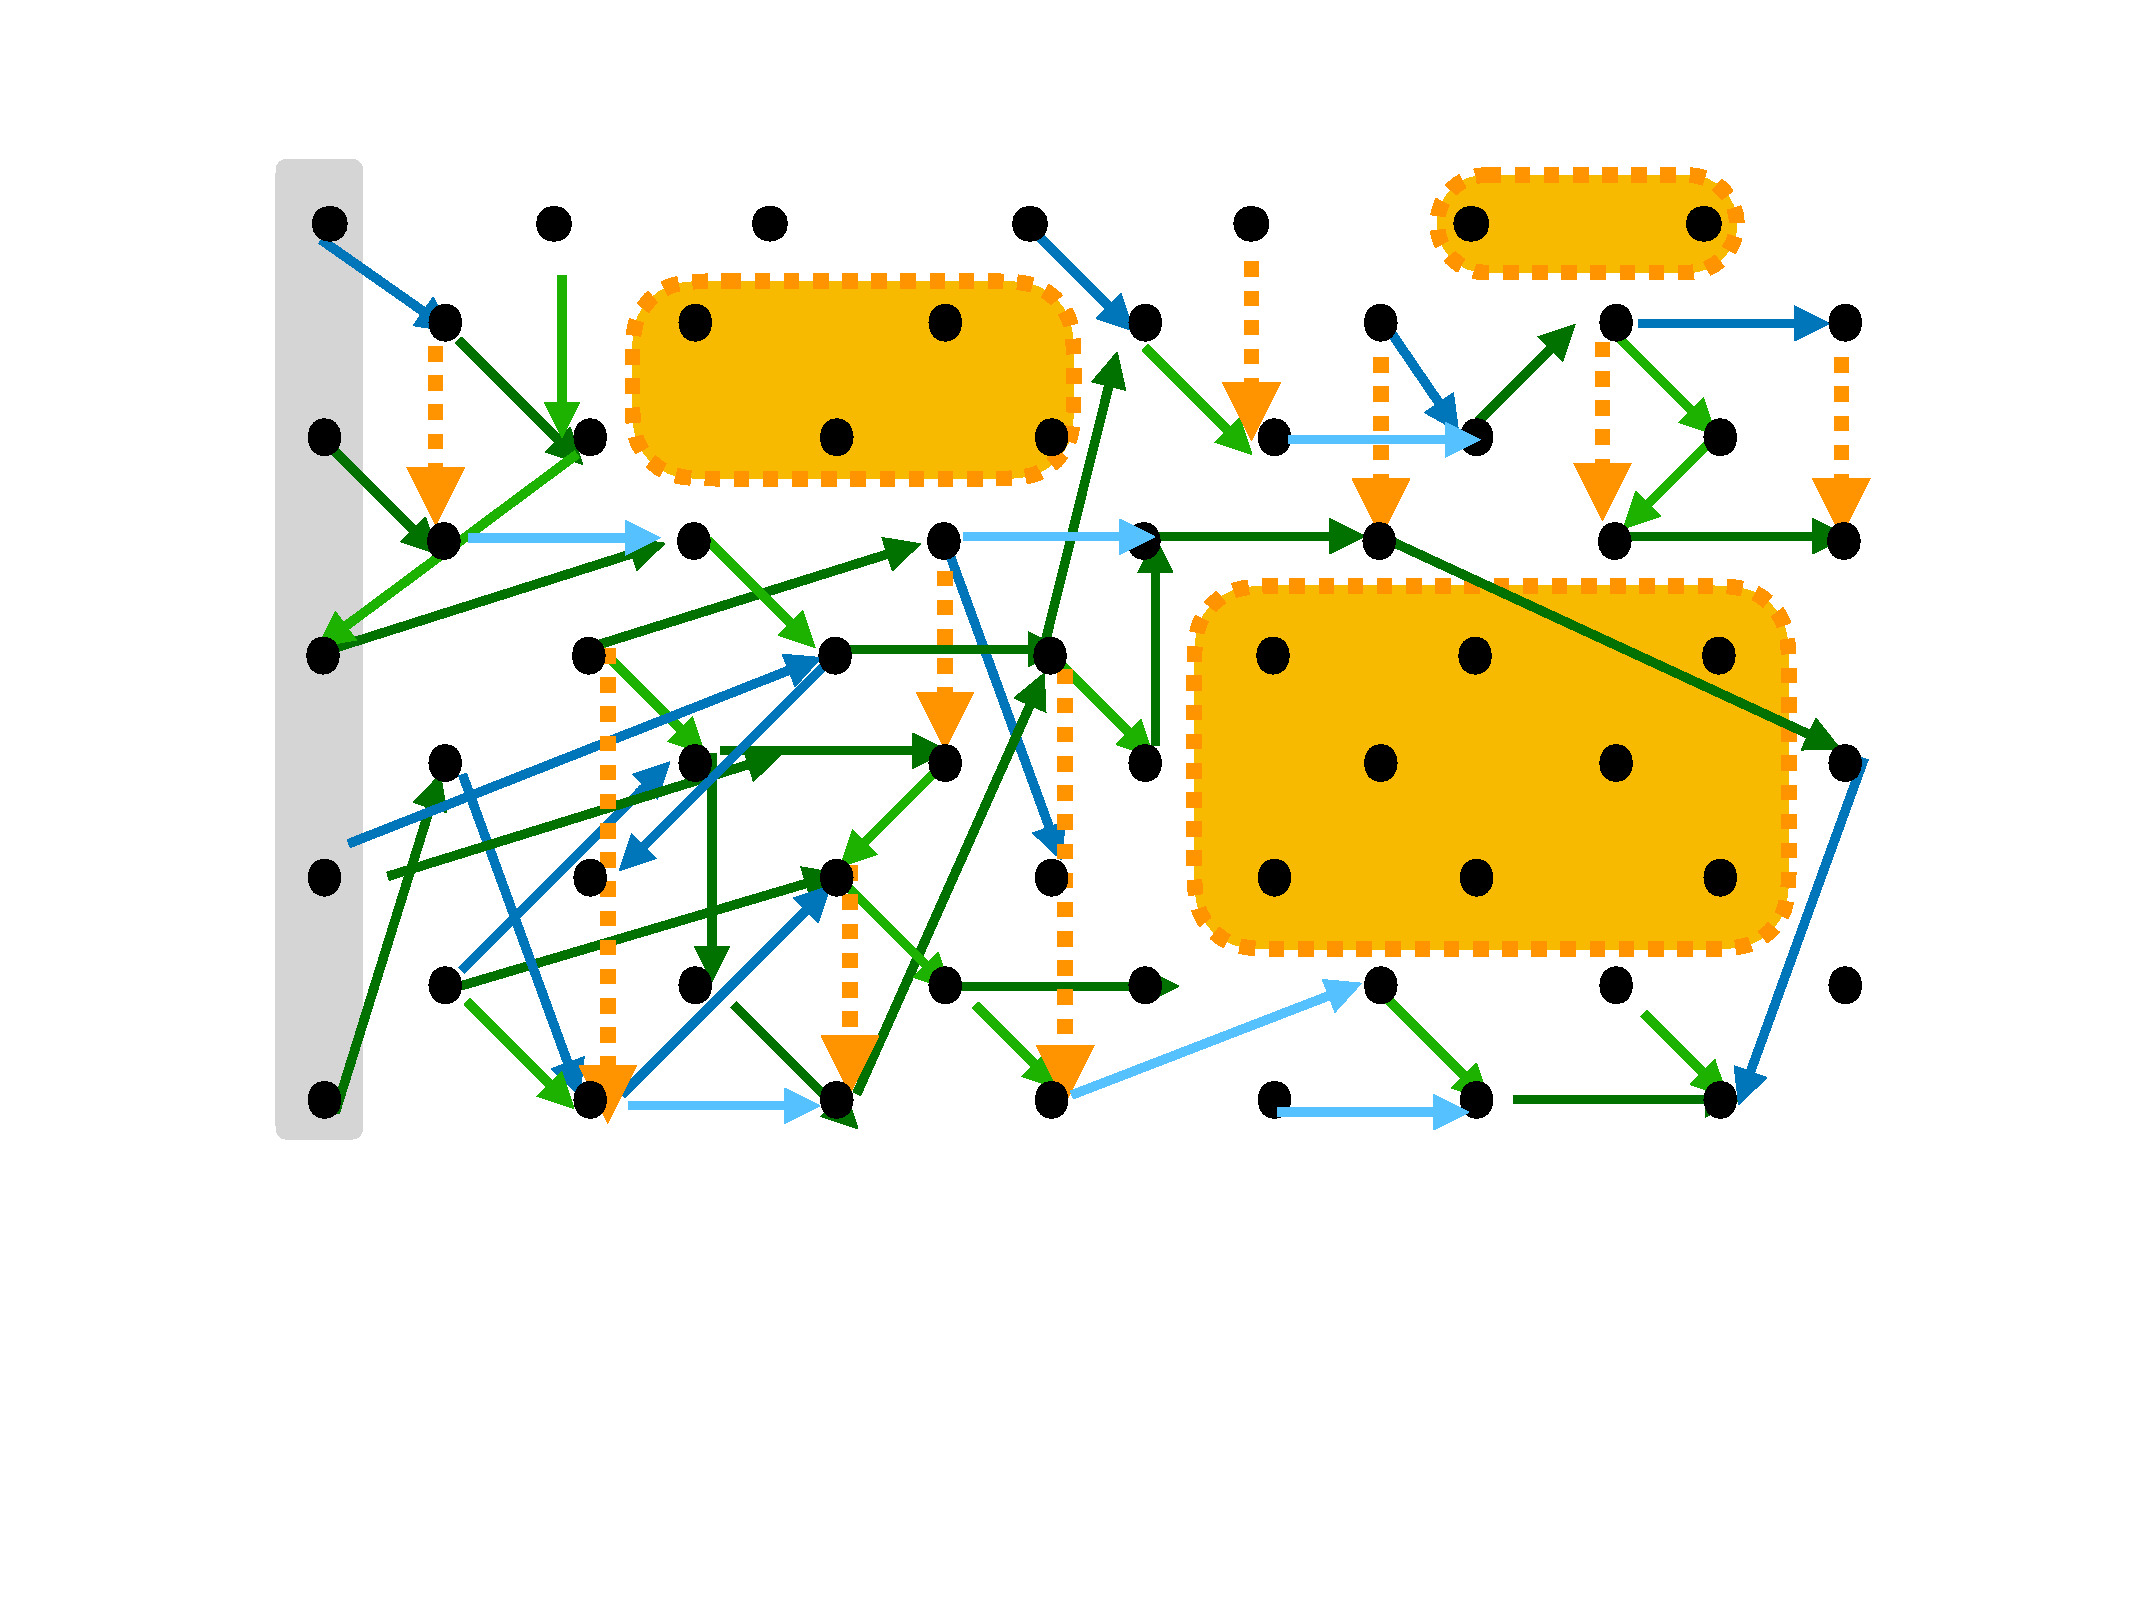
\includegraphics[width=\linewidth, trim=100  120 130 60,clip]{diagrams/neccSuffYellowAllExtended.pdf}
%%  \end{minipage}
%% \\
%% (a) sufficient  spec.& & (b) necessary spec. & & (c) full, holistic spec.
%% %\begin{minipage}{0.75\textwidth}
%% %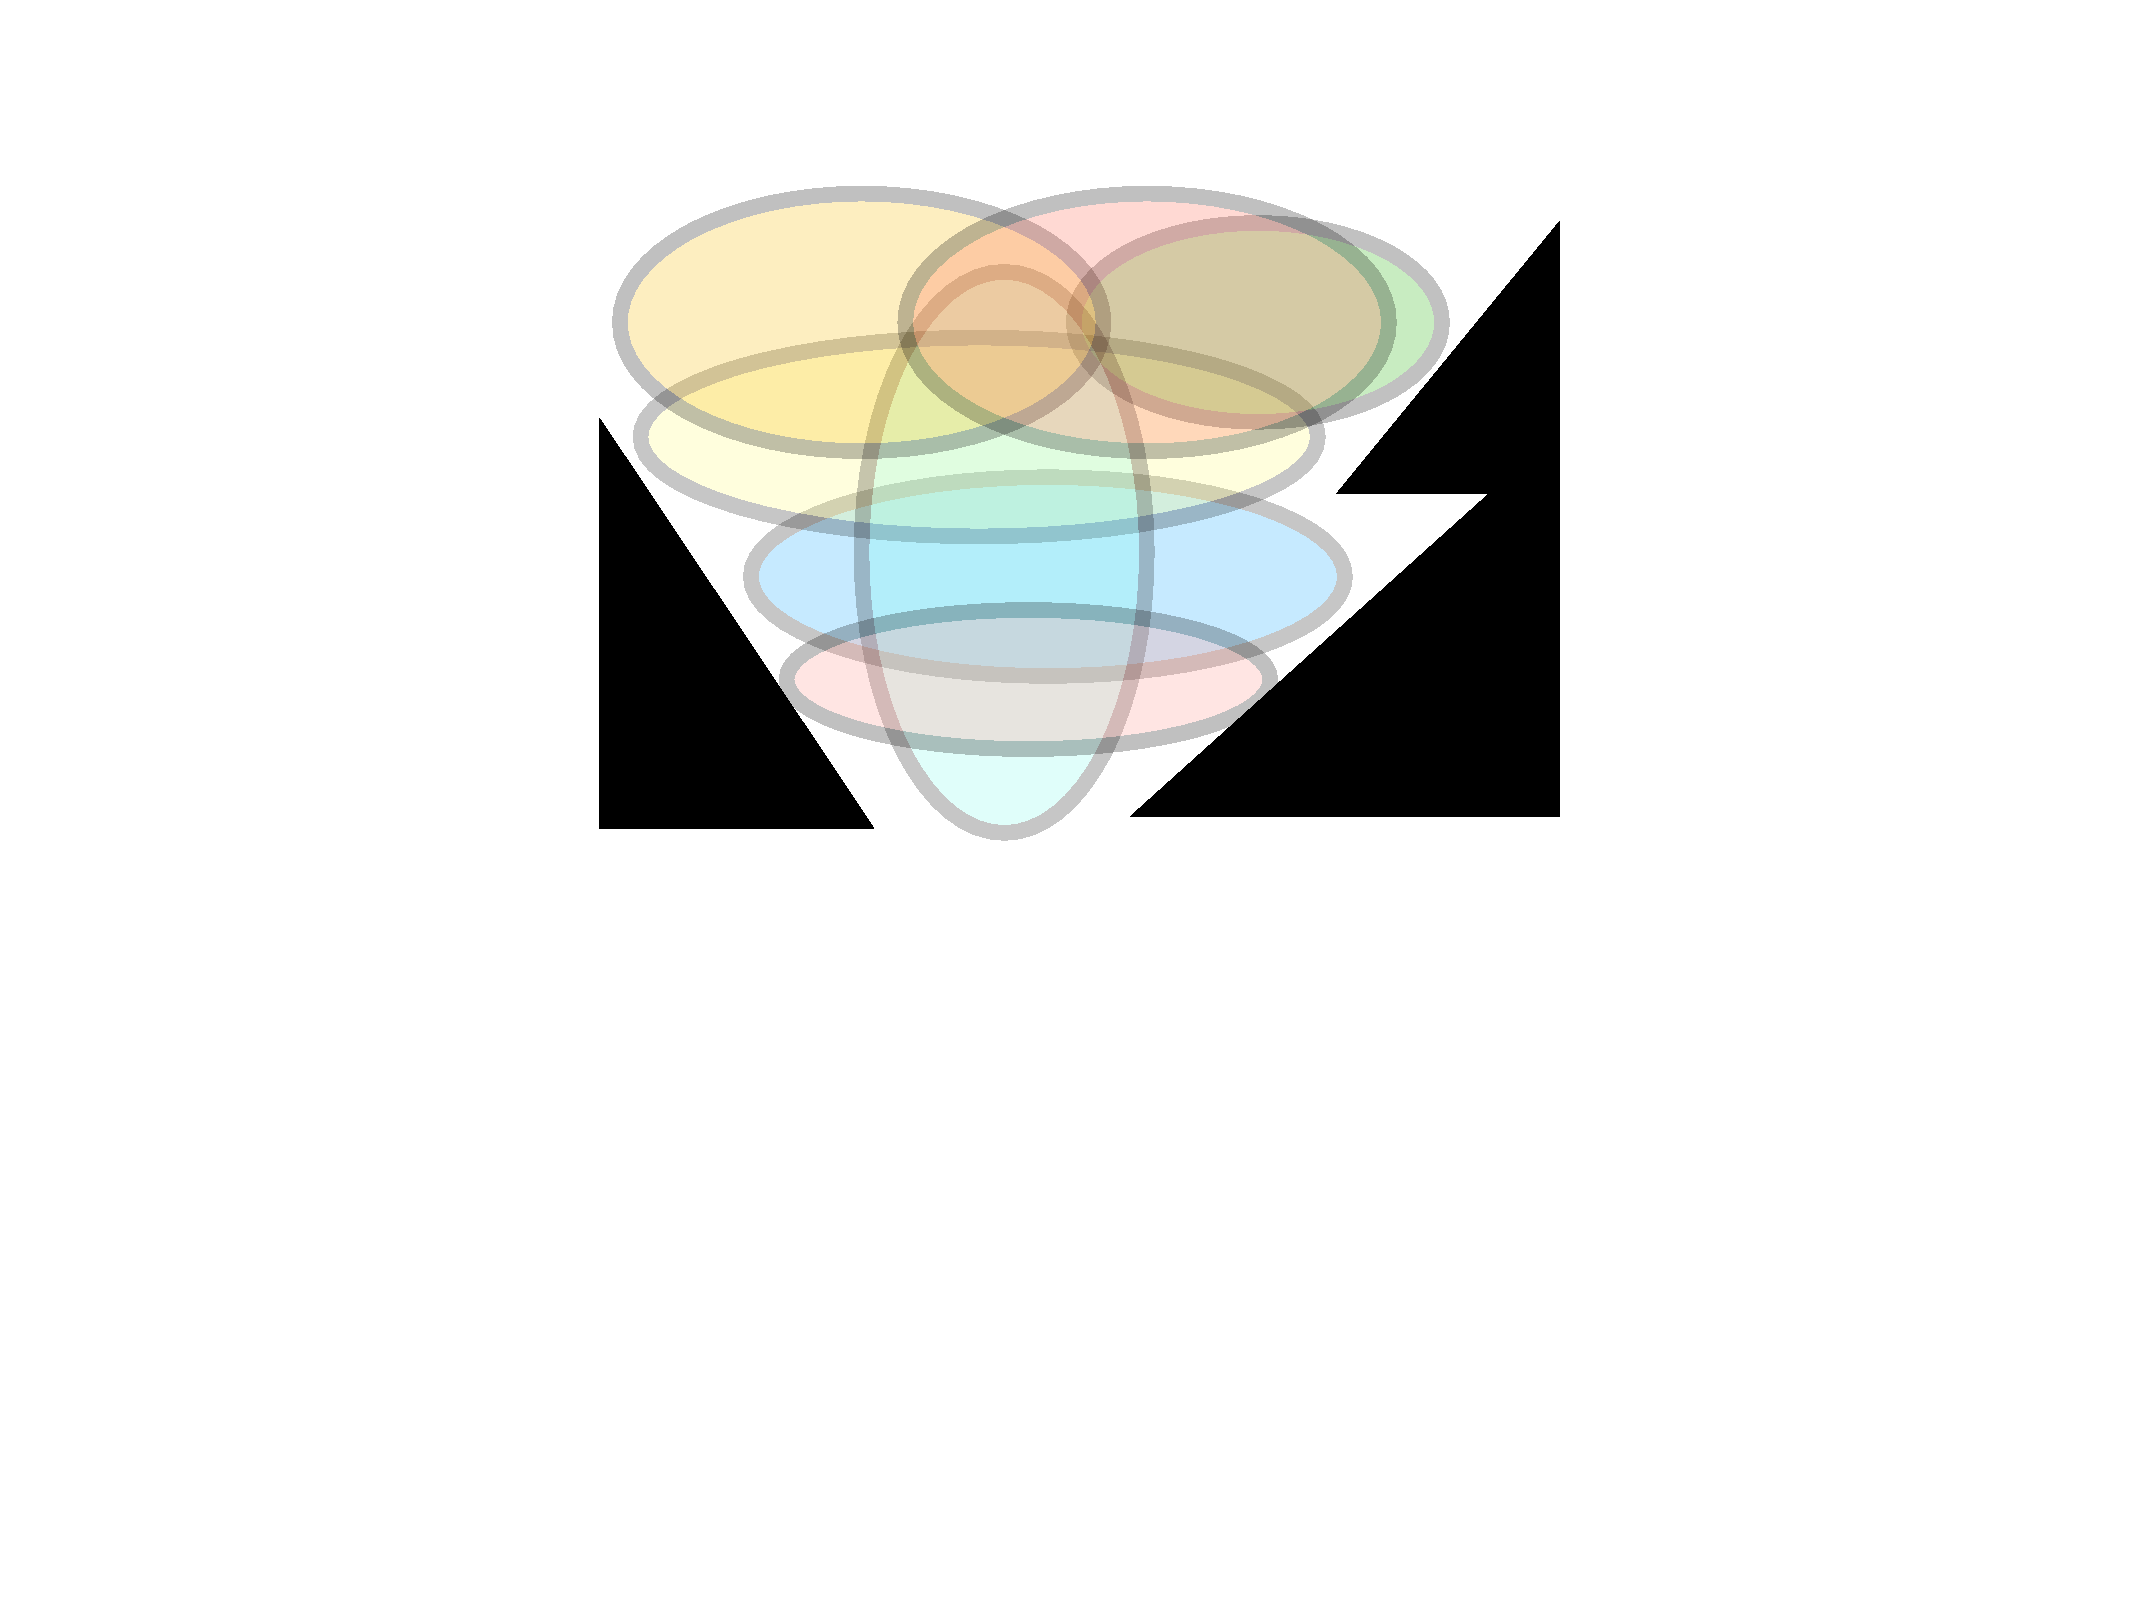
\includegraphics[width=\linewidth, trim=145  320 60 105,clip]{diagrams/NecAndSuff.pdf}
%% %\end{minipage}
%% %% y seems to eat up the bollom
%% %% x eats space from left, if you increase it the diagram decreases from left
%% %% w eats space from top, if you increase it the diagram decreases from top
%% %%\includegraphics[page=3, width=\linewidth, trim=150  270 40 150, clip]{diagrams/snmallocf.pdf}
%% %\sdcomment\sophia{I think we need to change the diagram so that it says small slab.}
%% %\end{minipage}
%%  \end{tabular}
%%   \vspace*{-2.5mm}
%%   \caption{Sufficient Conditions, Necessary Conditions, and Full Specifications}
%%  \label{fig:NecessaryAndSuff}
%%  \end{figure}
 
 We propose that  necessary conditions should be stated
 explicitly. Specifications should be \emph{holistic}, in the sense
 that they describe the  overall behaviour of a component: not only the
 behaviour of each individual function, but also limitations on the
 behaviour that emerges through combinations of functions.
%
Holistic specifications must therefore address sufficient as well as necessary conditions.
In   part (c)    in Fig. \ref{fig:NecessaryAndSuff} we show the 
immediate consequence of putting together assertions from necessary and sufficient conditions: 
there are no transitions from or to yellow boxes.

When a component satisfies its holistic specification,
% used to say "has been specified holistically" but this is not sufficient
then the states  in the yellow boxes and the 
behaviours
represented  by the yellow arrows cannot occur, even when the
component interacts with other software of unknown provenance.
(In Section \ref{sect:discussion} we argue why necessary conditions are more than the complement of
sufficient conditions.

 
Necessary conditions are guarantees upheld throughout program execution.
Therefore, they are close to monitor or object
invariants \cite{Hoare74,Meyer97}. The difference between 
classical invariants and our holistic specifications is that classical invariants  reflect  on
the current program state (\ie the contents of the
stack frame and the heap for an individual program component) while
holistic specifications reflect on all aspects of a program's
execution, potentially across all the components making up that program.


In this paper we propose \Chainmail, a specification language to
express holistic specifications.
The design of \Chainmail was guided by the study of a sequence of
examples from the object-capability literature and the smart contracts world: the
membrane \cite{membranesJavascript}, the DOM \cite{dd,ddd}, the Mint/Purse \cite{MillerPhD}, the Escrow \cite{proxiesECOOP2013}, the DAO \cite{Dao,DaoBug} and
ERC20 \cite{ERC20}.  As we worked through the
examples, we found a small set of language constructs that let us
write holistic specifications across a range of different contexts.
%
While many individual features of \Chainmail can be found in other work, 
their power and novelty for specifying open systems lies in their careful combination.
In particular, \Chainmail extends 
traditional program specification languages \cite{Leavens-etal07,Meyer92} with features which talk about:
%
\begin{description}
\item[Permission: ] 
%\ \ \textbullet \ \emph{Permission}, \ie
Which objects may have access to which other objects; 
this is central since access to an object usually also grants access to the functions it provides.
%
\item[Control: ]
%\ \ \textbullet  \ \emph{Control}, \ie
Which objects called functions on other objects; this
 is useful in identifying the causes of certain effects - eg 
funds can only be reduced if the owner called a payment function.
%
%$\bullet$ \ \\emph{Authority}, \ie which objects' state or properties may change; this is useful in describing effects, such as reduction of funds.
%
\item[Time: ]
%\ \ \textbullet \ \emph{Time}:\ \ie
What holds some time in  the past, the future, and what changes with time,
\item[Space: ]
%\ \ \textbullet \ \emph{Space}:\ \ie
Which parts of the heap are considered when establishing some property, or when 
performing program execution; a concept
related to, but different from, memory footprints and separation logics,
\item[Viewpoint: ]
%\ \ \textbullet \ \emph{Viewpoints}:\ \ie
%a distinction between the objects internal to our component, and those external to it;
Which objects and which configurations are internal to our component, and which  are
external to it;
a concept related to the open world setting.
\end{description}

Holistic assertions usually employ several of these features. They often have the form  of a guarantee
that only if some property holds now will a certain effect occur in the future, or that
certain effects can only be caused if another property held earlier.
For example, if within a certain heap (space) some change is possible in the future (time), then this particular heap 
(space again) contains 
at least one object which has access (permission) to a specific other, privileged object.
%\james{moved around --- not sure we need this para}
%\susan{I think we don't so there is a paragraph I have commented out.}
\forget{Often, holistic assertions typically have the form of a guarantee
that if some property ever holds in the future, then some other property holds now.
For example, if within a certain heap some change is possible in the future, then this particular heap contains 
at least one object which has access to a specific other, privileged object.}
A module satisfies a holistic assertion if  
 the assertion is satisfied  in all runtime configurations reachable through execution of the combined code of our module and any other module.
  This reflects the open-world view.


The contributions of this paper are:
\begin{itemize}
\item the design of the holistic specification language \Chainmail,
\item the semantics of \Chainmail,
\item a validation of \Chainmail through its application to a sequence of examples.
%\item a further validation of \Chainmail through informal proofs of adherence of code to some of these specifications.
\end{itemize}  
  
  
The rest of the paper is organised as follows: Section~\ref{sect:motivate:Bank} 
motivates our work via an example, and then
section~\ref{sect:chainmail} presents the \Chainmail\ specification
language.  Section~\ref{sect:formal} introduces the formal model
underlying \Chainmail, and then section~\ref{sect:assertions} defines
the 
semantics of \Chainmail's assertions.
% SD the below is NOT ture
%full details are relegated toappendices.   
Section~\ref{sect:example} shows how key points of 
exemplar problems can be specified in \Chainmail,
section~\ref{sect:discussion}
discusses our design, \ref{sect:related} considers related
work, and section~\ref{sect:conclusion} concludes.
We relegate various details to appendices.
